% !TeX spellcheck = en_US
% !BIB TS-program = biber
\documentclass[11pt]{article}

\usepackage{amssymb} % see: http://milde.users.sourceforge.net/LUCR/Math/mathpackages/amssymb-symbols.pdf
\usepackage{mathtools} % for extended mathematical symbols and more

% Page properties :
% See : https://tex.stackexchange.com/questions/36085/latex-without-pages
\usepackage{geometry}
\geometry{margin=25mm}

% Input file encoding :
\usepackage[utf8]{inputenc}

\usepackage[english]{babel}
\usepackage{lipsum}

\newcommand\BS{\char`\\}

\usepackage{caption}

\usepackage[
backend=biber,
style=numeric,
sorting=none
]{biblatex}
\usepackage{csquotes}
\addbibresource{Bibliography.bib}

% To color text :
% see : https://en.wikibooks.org/wiki/LaTeX/Colors
\usepackage[dvipsnames]{xcolor}


% Verbatim blocks :
\usepackage{verbatim} % normal verbatim
\usepackage{fancyvrb} % for fancy boxed varbatims
\usepackage{parskip}


% To use images : 
\usepackage{graphicx} % use this
\graphicspath{ {./IMG/} } % path midifier for storing images
% to include a picture, type this ('name' is without path or extention) :
% \includegraphics[width=0.5\textwidth]{name}

\usepackage{dirtytalk}
\usepackage{parskip}

% How to use references :
\usepackage{hyperref} % use this
\hypersetup{
	colorlinks=true,    
	urlcolor=blue,
	citecolor=black
}

\usepackage{wasysym}

\usepackage{color}
\definecolor{mylightgray}{rgb}{0.95,0.95,0.95}
\definecolor{mygreen}{rgb}{0,0.6,0}
\definecolor{mygray}{rgb}{0.5,0.5,0.5}
\definecolor{mymauve}{rgb}{0.58,0,0.82}

\usepackage[super]{nth}

% Regulates \tableofcontents max depth
\setcounter{tocdepth}{2}

\usepackage{array}
\newcolumntype{L}[1]{>{\raggedright\let\newline\\\arraybackslash\hspace{0pt}}m{#1}}
\newcolumntype{C}[1]{>{\centering\let\newline\\\arraybackslash\hspace{0pt}}m{#1}}
\newcolumntype{R}[1]{>{\raggedleft\let\newline\\\arraybackslash\hspace{0pt}}m{#1}}
\usepackage{xcolor,colortbl}
\newcolumntype{a}{>{\columncolor{mylightgray}}l}


\usepackage{listings}
\lstset{ 
	backgroundcolor=\color{mylightgray},   % choose the background color; you must add \usepackage{color} or \usepackage{xcolor}; should come as last argument
	basicstyle=\small,        % the size of the fonts that are used for the code
	breakatwhitespace=false,         % sets if automatic breaks should only happen at whitespace
	breaklines=true,                 % sets automatic line breaking
	captionpos=b,                    % sets the caption-position to bottom
	commentstyle=\color{mygreen},    % comment style
	deletekeywords={...},            % if you want to delete keywords from the given language
	escapeinside={\%*}{*)},          % if you want to add LaTeX within your code
	extendedchars=true,              % lets you use non-ASCII characters; for 8-bits encodings only, does not work with UTF-8
	firstnumber=1,                % start line enumeration with line 1000
	frame=single,	                   % adds a frame around the code
	keepspaces=true,                 % keeps spaces in text, useful for keeping indentation of code (possibly needs columns=flexible)
	keywordstyle=\color{blue},       % keyword style
	%language=Java,                 % the language of the code
	morekeywords={},            % if you want to add more keywords to the set
	numbers=none,                    % where to put the line-numbers; possible values are (none, left, right)
	numbersep=5pt,                   % how far the line-numbers are from the code
	numberstyle=\tiny\color{mygray}, % the style that is used for the line-numbers
	rulecolor=\color{black},         % if not set, the frame-color may be changed on line-breaks within not-black text (e.g. comments (green here))
	showspaces=false,                % show spaces everywhere adding particular underscores; it overrides 'showstringspaces'
	showstringspaces=false,          % underline spaces within strings only
	showtabs=false,                  % show tabs within strings adding particular underscores
	stepnumber=2,                    % the step between two line-numbers. If it's 1, each line will be numbered
	stringstyle=\color{mygreen},     % string literal style
	tabsize=2,	                   % sets default tabsize to 2 spaces
	title=\lstname                   % show the filename of files included with \lstinputlisting; also try caption instead of title
}
\usepackage[multiple]{footmisc}

\usepackage{wrapfig}

\usepackage{multirow,booktabs} % https://jdhao.github.io/2019/08/27/latex_table_with_booktabs/

\usepackage{array}
\setlength\extrarowheight{4pt}

\newcounter{codeID}[section]
\newcommand{\nextcodeID}{\refstepcounter{codeID}\multirow{3}{*}{\thecodeID}}

\usepackage{longtable}

\newcommand{\degrees}[1]{#1$^{\circ}$}

%% Define a HUGE : https://tex.stackexchange.com/questions/265/fonts-larger-than-huge
\usepackage{fix-cm}   
\makeatletter
\newcommand\HUGE{\@setfontsize\Huge{29}{35}}
\makeatother 

%% Adds padding to tables : https://tex.stackexchange.com/questions/64761/add-just-a-little-more-padding-to-my-table/381439
\usepackage{array}
\setlength\extrarowheight{2pt} % or whatever amount is appropriate

\usepackage{authblk}%[affil-it]
%opening
\title{\vspace{15mm}{\HUGE PoGER : a game engine recreation and software preservation project}\\[4mm]
	A Bachelor's project}
\author{David Rodriguez Soares}
\date{}
\affil{Centre Universitaire d'Informatique,\\University of Geneva, Switzerland}

% first page
\begin{document}
\maketitle

\vfill
%
\section*{Abstract}

Game development has evolved from an obscure activity only teams of people with specialized training could work on to an accessible art through the use of powerful tools and shared already-made code and assets, springing a healthy and successful independent game-making scene. Unfortunately, this is not the state of most fan-made game creation communities, in particular the one dedicated to the popular Pokémon franchise. It is plagued by a combination of issues, mainly the inadequacy of used tools and software preservation challenges.

This paper presents PoGER, an software preservation and game engine recreation project aimed at proposing systemic solutions to these issues. We discuss the goals of this project, the reverse-engineering effort, its findings and design decisions taken. We also present a framework and tools for both porting old projects and facilitating future development, which could kickstart a new wave of enthusiasm in its field and hopefully give motivated developers an opportunity to create their own worlds and adventures.


\newpage

\begingroup
\hypersetup{linkcolor=black}
\tableofcontents
\endgroup
%
%\newpage




%This is intended to document my journey through my Bachelor's project. Some information may be omitted for brevity or because it is present in accompanying scripts.

%It can be decomposed \textbf{3 major steps} : \textit{inception}, \textit{research} and \textit{implementation}.

%\subsection{Related documents}
%
%This is but one in a collection of manuscripts, each with its scope (\textit{sorted older to newer}) :
%
%\begin{itemize}
%	
%	\item \textbf{Vision document} : A very early analysis about Pokemon Essentials, focused on identifying its issues and properties of a hypothetical software solution.
%	
%	\item \textbf{\textit{PoGER}} : Gives information on the project itself, including motivations and objectives.
%	
%	\item \textbf{RMXP doc} : Contains the results of my research about RPG Maker XP's implementation of game data (mostly \textit{Maps} and \textit{Events}), with the objective to extract them to an interpretable format.
%	
%	\item \textbf{Extraction} : Contain a practical guide on the extraction process for anyone trying to reproduce it.
%\end{itemize}


%\subsection{Notes}
%
%Here are some of the abbreviations you can encounter :
%\begin{itemize}
%	\item \textbf{RMXP} - RPG Maker XP
%	\item \textbf{RGSS} - Ruby Game Scripting System
%	\item \textbf{PE} - Pokemon Essentials
%	\item \textbf{PU} - Pokemon Uranium
%\end{itemize}
%
%Please note that the author is not a native English speaker.


\newpage
\section{Introduction}

Since its creation by japanese game designer  Satoshi Tajiri in 1995 \cite{PkmnCreator,SatoshiBook}, the Pokémon franchise (also known as \textit{Pocket Monsters} in Japan) had a significant impact on culture around the world \cite{PkmnPop,PkmnEffect} and on its own genre (the JRPG, for Japanese Role-Playing video Game) \cite{PkmnRPG}.

The Pokémon games, originally launched on the Nintendo Game Boy handheld, experienced immediate and global success, selling over 46 (or 31 if not counting \textit{Pokémon Yellow}) million units on its first generation \cite{PkmnSales} and more than 368 million copies sold overall \cite{PkmnFigures}.

\begin{figure}[!h]
	\centering
	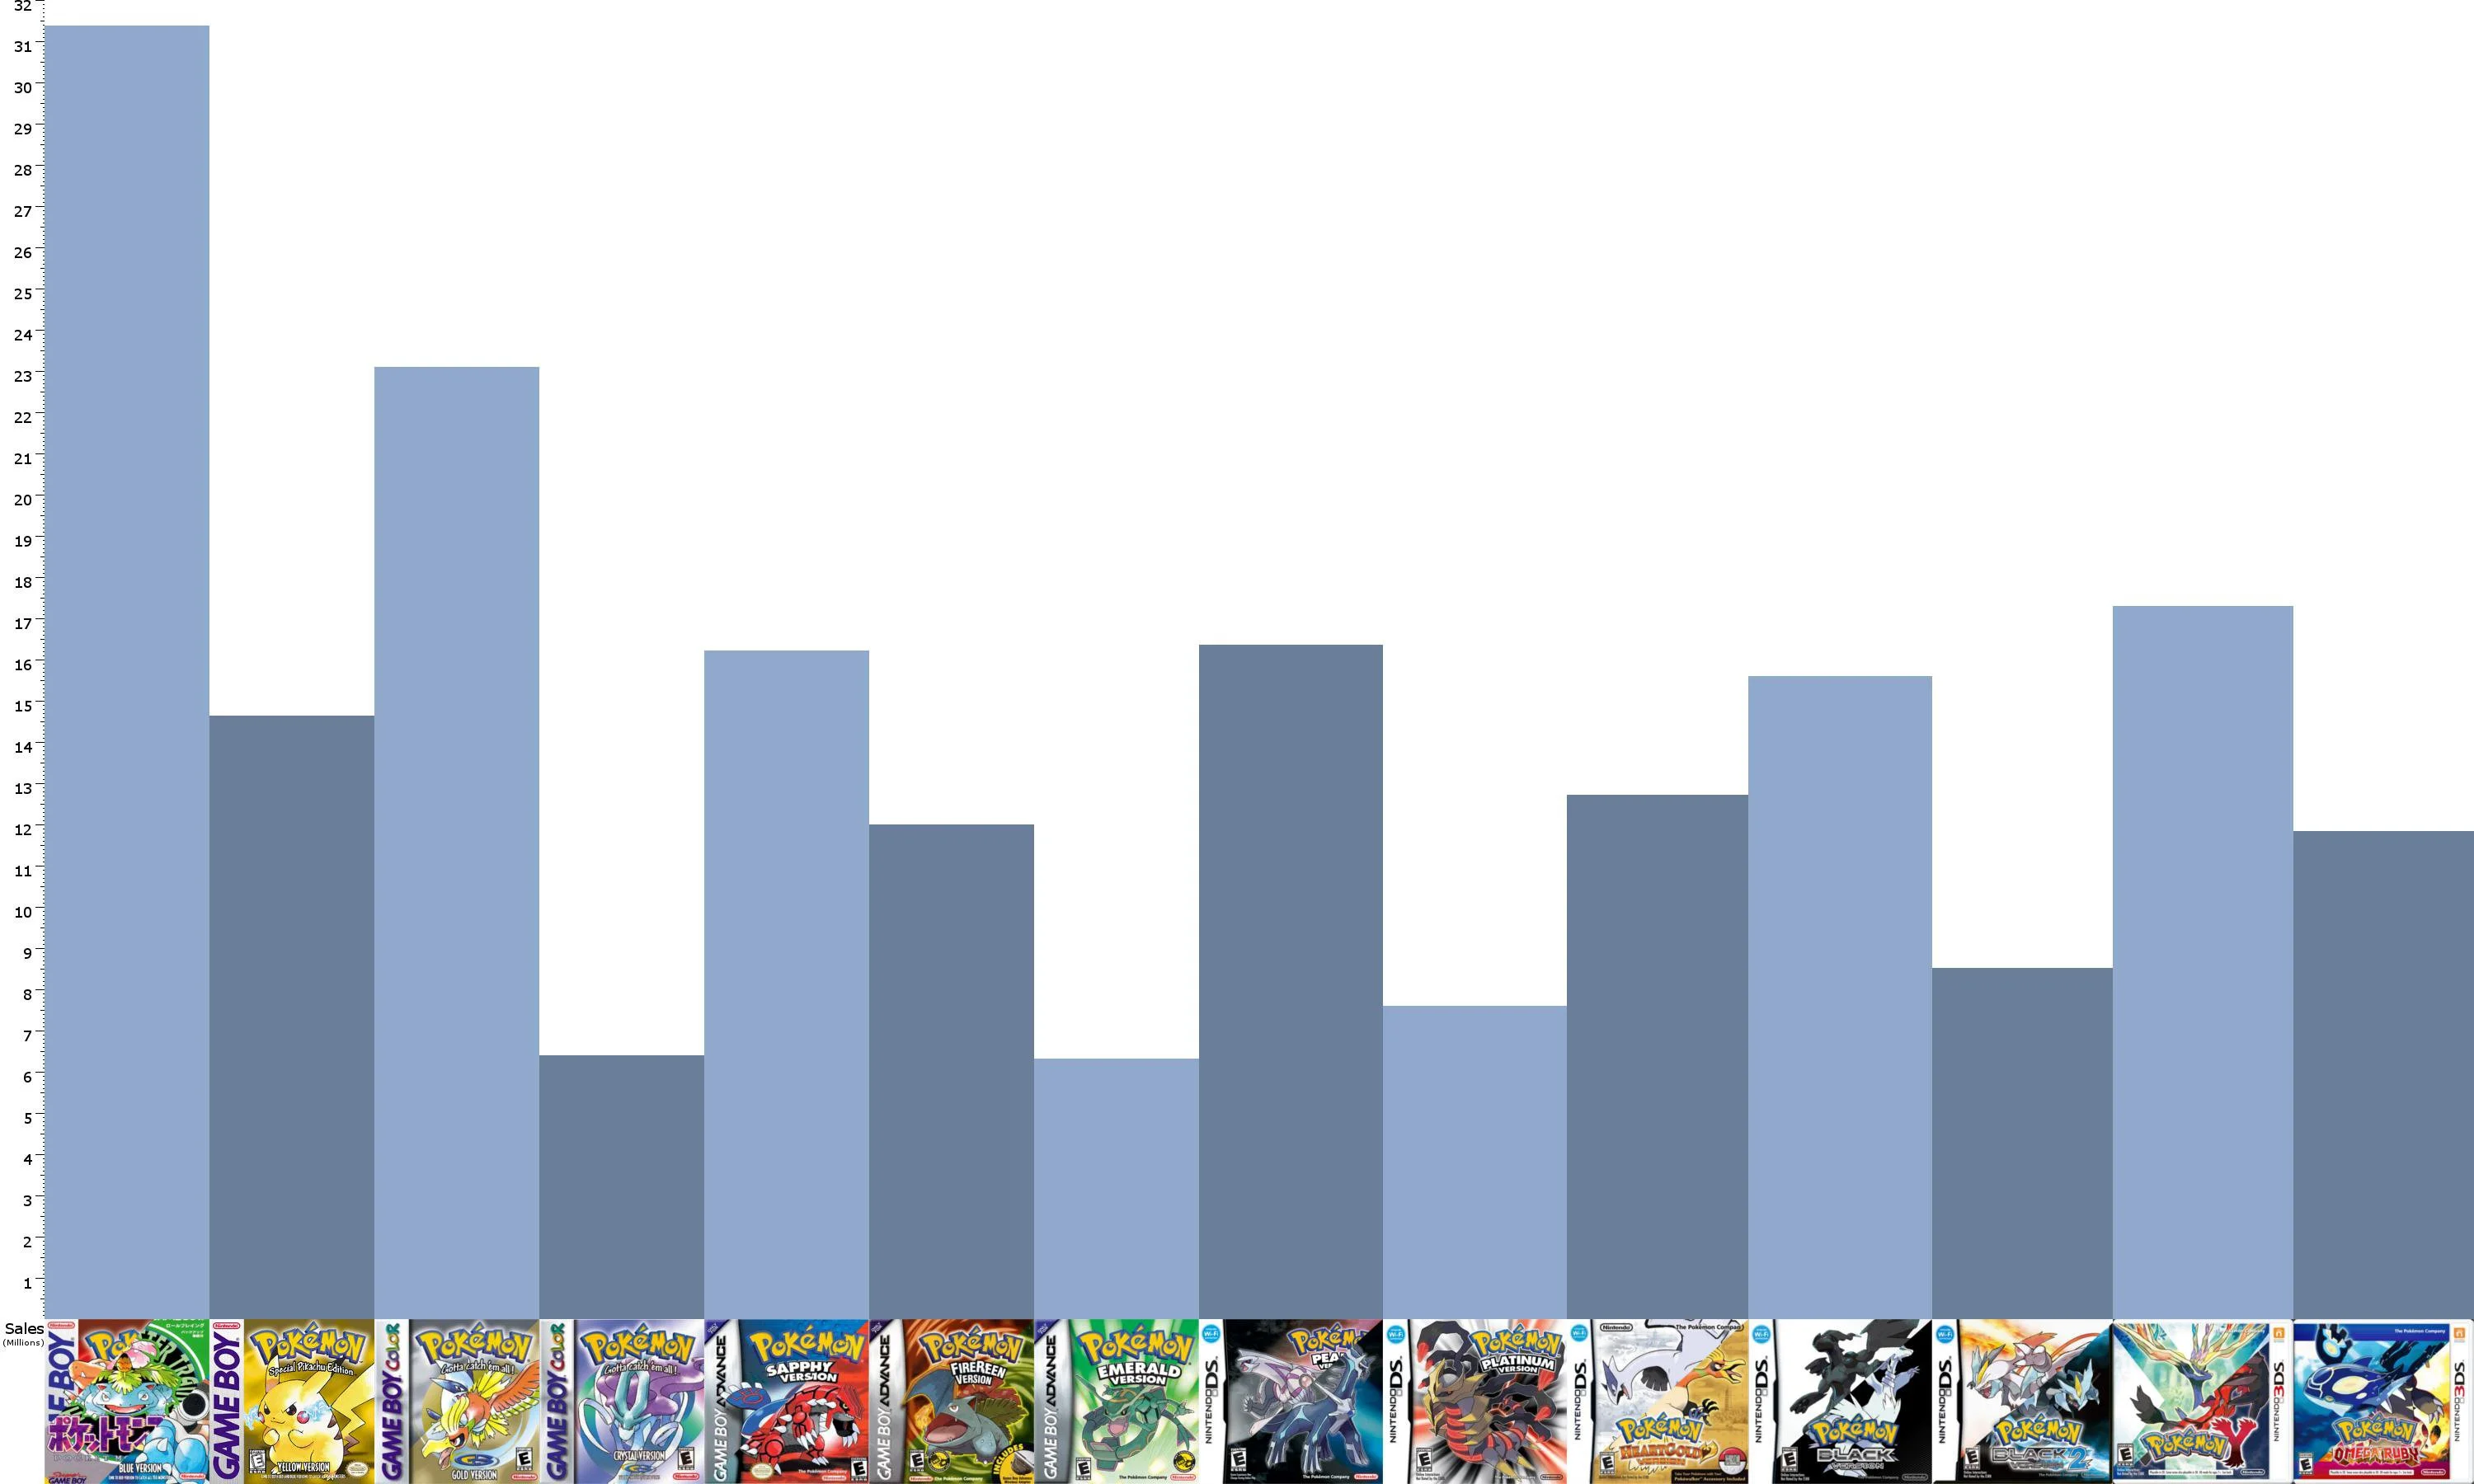
\includegraphics[width=\textwidth]{Pokemon_sales_gen}
	\caption{Unit sales of Pokémon mainline games, in millions \cite{PkmnSales,PkmnSalesIll} }
\end{figure}

Since then, it influenced generations of people who created art \cite{PkmnArt}, named animals and proteins \cite{Pikachurin,Etymology}, wrote novels \cite{Novel}, did scientific research, etc. Simply search for \texttt{Pokémon} on an academic search engine like \texttt{Google Scholar} and you would be surprised of the amount of results and the diversity of represented fields !

With such a motivating and long-running game franchise, it was inevitable some fans would look into the possibility of making their own addition to the series.

\subsection{The state of Pokémon fan-made games}

As the name suggest, these games are created by fans of the franchise and are based on its core concepts and gameplay mechanics \cite{PkmnFangames}. Over the last two decades, many game projects saw a release on the Internet and even a few can be found in physical media form \cite{PkmnUV,PkmnCartridge} !

But what does that development scene looks like ? What we discovered is a clustered universe of fan-made games. There are 3 main categories : 

\textbf{ROM hacks} \ Build upon the code and assets of commercial products, typically GameBoy games \cite{PkmnFangames}, they can be played on common emulators (and on original hardware \cite{Homebrew}), therefore available for most platforms. Unfortunately, programming for them is very technical, with limited functionality and questionable legality \cite{PkmnRH}.

\textbf{Games made with RPG Maker XP} \ Build on top of the \textit{Pokemon Essentials} project \cite{PkmnFangames,Essentials}, they are easier to program for and have less limitations than ROM hacks.

\textbf{Original games} \  These are original software, typically built for Windows or the web. Thanks to that, they can have great performance and novel game mechanics (eg. MMORPG style), but remain typically closed-source, and only a few projects exist \cite{PkmnPlanet, PkmnLegends, PkmnFanGameList}.


\subsection{Problems}

% Problématique

A lot of people tried to make their own games by love for the franchise, but from my early research into Pokémon fan-made games, a few common issues can be identified.

Except for ROM hacks and the occasional web-based game, which run on emulators and web browsers respectively, software is \textbf{platform-specific} (typically made for the Windows operating system). This is not optimal, because it restricts the amount of devices they can be run on, thus their market. Combined with the fact that they are almost universally \textbf{closed-source}, it becomes an issue of \textbf{software conservation}.

Another common issue is the \textbf{high amount of technical knowledge} that anyone willing to work on them needs, even with tools like RPG Maker XP.

Due to the \textbf{legality challenges} and the \textbf{personal nature} of fan-games, but also the \textbf{lack of collaborative code source management tools} (like \textit{git}), they are typically a \textbf{single-developer endeavor}. 

The combination of previously mentioned issues is, in my opinion, a perfect storm that explains the lack of quality fan-made games in a time independent game development is on the rise : It kills most attempts before they are release-worthy and keeps the rest from ever becoming polished and rid of bugs as commercial games. 

This happens because their developer finds no more time to invest or lose interest in them, and picking them up once that happened can be incredibly difficult, or even impossible.

This was an indication there was a need for a solution that would address these issues, but we knew it was unrealistic to do so for every category of games. 


\subsection{Focusing on Pokemon Essentials}

\textit{See Section 3 for more detailed information.}

RPG Maker XP is an popular but aging RPG engine that offers convenient tools that allows anyone to make their own role-playing video game \cite{RMXP}.

Unfortunately, programming for it is technical and it's only natively compatible with Windows. Note that compatibility layers such as Wine on GNU/Linux are able to launch games made with it such as \texttt{Pokémon Uranium} \cite{LutrisPU}. Also, performance is typically poor due to its aging engine \cite{PoorPerf}.

\textbf{Pokemon Essential} is a project that aims at offering an implementation of the Pokemon game engine that runs on RPG Maker XP. Few projects using it were completed \cite{PkmnFangames}.

Even with the facilities introduced, programming for RPG Maker XP/Pokemon Essentials remains complex, and is typically done in very small teams of amateurs, not using collaborative source code management tools like \textit{git}. This results in ambitious project requiring years before they can be released and are hard to maintain (see \texttt{Section 3.3} for a case study).

We believe this is the reason most projects never see a release, and the ones that do are buggy.


\subsection{Defining the project}

%We started by identifying shortcomings of the studied software, then moved on to coming up with solutions.

Problem definition : RPG Maker XP/Pokemon Essentials isn't adapted to creating a game in a modern way, and suffers from its age and design decisions, and unfortunately there doesn't seem to be a superior alternative tool for the purpose of creating a Pokemon game. Also, games based on these tools present significant software preservation challenges.

Further research made it clear that we should not try to build upon it, but rather bring it up somehow.

%We won't detail every design decision here, but each one was made toward the goal of addressing the identified shortcomings of the studied software. Please read the \textit{vision document} for more information.

The solution we came up with : implementing an engine functionally similar to Pokemon Essentials that would be decoupled from RPG Maker XP  and would run games as programs written in an interpreted domain-specific language we would create. A complementary piece of software would automate the port of games written for the original Pokemon Essentials engine, therefore satisfying our goals of software preservation and making it more relevant than an alternative without any retro-compatibility path.

There is a name for this approach : \href{https://en.wikipedia.org/wiki/Game_engine_recreation}{game engine recreation}.  That's where the name for this project comes from, \textbf{PoGER} (\textit{\textbf{Po}kémon Essentials \textbf{G}ame \textbf{E}ngine \textbf{R}ecreation}).

\textbf{Requirements} : A solution would be an implementation of Pokémon Essentials that : 
\begin{itemize}
	\item is performant
	\item is available (os independent)
	\item is straightforward and simpler to develop for
	\item has online capabilities
	\item has engine code separate from game code
	\item provides documentation, sets standards
	\item is fundamentally open-source to allow contributors to maintain projects.
	\item has a way to port games from the original Pokémon Essentials
\end{itemize}

\newpage
\subsection{Outline}

This report is divided in nine sections (\textit{plus reference list}), including this introduction.

\begin{itemize}
	\item Section 2 briefly explores the modern preoccupation of software perservation and discusses the application of its principles to the current project.
	
	\item Section 3 gives a detailed summary of identified software and projects of interest.
	
	\item Section 4 looks into the feasibility of asset and feature extraction from an existing Pokémon Essentials project. Then, it presents the implementation results of the extraction process and details the steps involved in a practical guide fashion.
	
	\item Section 5 presents the reverse-engineering results for a particularly complex category of extracted assets : Events. This is followed by a discussion on the necessity of a new representation for them and the design decisions behind the proposed domain-specific language. A formal definition is given, with examples and a Python implementation.
	
	\item Section 6 presents the early work on \texttt{PEN}, an interpreter that can run events. This would be the basis for an interpreter capable of running a full game. A portion is dedicated to PBS files and information that can be imported from them.
	
	\item Section 7 covers the reverse-engineering efforts aimed at interpreting RPG Maker XP's proprietary map and map asset format. Then, it presents a proof of concept implementation in Python.
	
	\item Section 8 explores the future of the project, the path towards an actual implementation of an interpreter capable of executing games, providing directions for future work.
	
	\item Section 9 closes this report with a summary and a critique of its contributions.
\end{itemize}


\subsection{About unincluded assets}

For practical reasons, a few elements couldn't be included in this document. These are mainly the software produced for the purpose of demonstration, proofs of concept, etc. Any referenced document/directory/file that isn't located in an \texttt{Appendix} shall be available in the following GitLab repository :

\begin{center}
	\texttt{https://gitlab.unige.ch/David.Rodriguez.1/poger}
\end{center}





\newpage

\section{About software preservation}

\textit{Digital preservation} describe the efforts aimed at insuring access to digitally stored information and the strategies, technologies and actions involved in resolving the challenges said effort comes across \cite{digipresdef,lee2002state}. This is a broad endeavor that spawned multiple projects with different scopes.

A common scope for digital preservation is \textit{web archival}, which aims at insuring access to web pages long after their content is changed or rendered inaccessible \cite{masanes2006web}. A well known service implementing web archival is the \texttt{Wayback Machine} \footnote[1]{https://web.archive.org/}, which enable anyone to visit a web page at a previously stored state given its address.

\textit{Software preservation} is mainly focused on insuring access to means of \textit{running software} and \textit{preserving source code}.


\subsection{Maintaining the ability to run software}

A modern preoccupation is the preservation of aging hardware and software, because as time passes, functional ancient hardware becomes increasingly scarce, and with it the means to run software made for it.

The problem of maintaining the possibility to run software despite the loss of access to its original platform pushed the development of \textbf{virtualization and emulation technologies}.

From \texttt{David S. H. Rosenthal's article} \cite{rosenthal2015emulation}:

\say{\textbf{Virtualization} is a technique for implementing a VM on a host computer. It depends on the host computer’s instruction set being the \textit{same} as [...] the VM’s instruction set, and having certain specific hardware properties that enable virtualization. Almost all instructions executed by the VM are directly executed by the host computer’s CPU; only a few instructions are intercepted, using the specific properties, and performed by host software. Virtualized systems run \textit{unmodified} software binaries.

[...]

\textbf{Emulation} is a technique for implementing a VM
on a host computer whose instruction set is \textit{different} from the host computer’s. None of the instructions executed by the VM are directly executed by the host computer’s CPU; all are translated by host computer software from the VM’s instruction set to the host computer’s instruction set by host software before being executed. Emulated systems run \textit{unmodified} software binaries.}

Both these technologies have a lot in common : software compatibility (the capacity of running software by matching compatible hardware interface), overhead (the additional computation necessary for the hardware abstraction) and isolation (the capacity of running software without impact on the host system) \cite{rosenblum2004reincarnation}. Most importantly, by abstracting the hardware expected from the software for it to be executed, it allows it to be executed on any hardware that implement these technologies.

In some instances, yet another strategy may be used : \textbf{Translation}. This is a technique to convert software from an archaic language to a modern one, therefore insuring its preservation in another form, but typically requiring its source code \cite{swalwell2009towards}.

Each approach has its benefits, drawbacks, scopes and challenges, therefore there isn't a universal approach to this aspect of software preservation.


\subsection{Preserving source code}

The long-term preservation of source code is motivated by the observation that software is omnipresent in our modern life, scientific research and enables access to digital information. As such, it can be conceived as a common good, another storage medium for \textit{knowledge}, therefore worth conservation \cite{di2017software}. Unfortunately, it presents unique challenges, including but not limited to :

\textbf{Availability} : Software in \textit{executable form} is unreadable by humans, and its \textit{source code} counterpart, which contains actual \textit{knowledge}, may not be available \cite{di2017software}. The rise of Free/Open Source Software (FOSS), founded on principles of source code accessibility, is therefore a welcome phenomenon \cite{schweik2012internet}.

\textbf{Artifacts} : Software development is a process that produces artifacts by its developers and users: documentation, change logs, guides, FAQs, issues discussion threads, etc. Such artifacts are of crucial importance and offer context about its software \cite{di2017software,corrado2019software}. Source code preservation projects may decide to include this knowledge.

\textbf{Mutability} : As a digital object, source code is bound to evolve over time, to the point of generating incompatibilities between different versions. Version management technologies are needed to capture its history and organize it in a comprehensive way \cite{di2017software,holzmann2016archiving}.


Source code has interesting particularities : It's hard/expensive to produce and compact in size. It follows that simply storing valuable amounts of it isn't technically or financially challenging, rather the capacity of presenting it in a useful way is. Various projects aiming at long-term software source code preservation are focused on developing archiving and cataloging technologies to offer effective access to their stored knowledge (not an exhaustive list) :

\begin{itemize}
	
	\item Software Heritage : Focuses on source code, indiscriminately of origin \cite{di2017software,softheri}.
	
	\item Zenodo : Focuses on data and software involved in scientific research. They use GitHub/GitLab integration for importing source code \cite{zenodo}.
	
	\item GitHub Archive program : A project with multiple well-known partners, with "very-long-term" archival objectives and a focus on storage technologies lifespan and redundancy \cite{githubap}
	
\end{itemize}




\subsection{Link with PoGER}

One of the goals of this project is to present a candidate framework for recovering source code, give it an alternative representation, insure the ability to execute it independently to its original platform and do so in a open-source-oriented fashion.




\newpage
\section{Research subjects}

In order to define the scope of this project, becoming familiar with the games and tools used to make them was a crucial step. In this section, we detail relevant information on RPG Maker XP/Pokémon Essentials and present a case study for a particular game : \texttt{Pokémon Uranium}

\subsection{RPG Maker XP}


According to its official website\footnote{https://www.rpgmakerweb.com/products/programs/rpg-maker-xp} and its Steam listing\footnote{https://store.steampowered.com/app/235900/RPG\_Maker\_XP/}, RPG Maker XP was developped by Enterbrain and released on July of 2004 for Microsoft Windows. 

It allows its users to create their own role-playing game with powerful dedicated tools and its engine is based on the Ruby programming language, making complex behavior possible through the use of \textit{scripts}.


This is only one instance among the long line of RPG Maker releases, some of which were released on other platforms, including consoles. Probably due to its early popularity, new projects continued to use this version way after it was superseded by newer ones.



\subsubsection{Ruby Game Scripting System}

From an article on this subject\footnote{https://rmvxace.fandom.com/wiki/RGSS} : 

\say{RGSS stands for Ruby Game Scripting System, a library that has been used in RPG Maker engines since RPG Maker XP.  It's a Ruby library, and as such, all scripting is done in the Ruby language.
	
In all of its incarnations, RGSS has included objects and methods with which to handle graphics, audio, and data, including basic data structures for the RPG Maker engine.

The original version, RGSS, [...] was based on Ruby 1.81.}

RGSS's latest version, RGSS3, was introduced with RPG Maker VX Ace in 2011-2012 \cite{rgssspec,rmvxacerelease}.






\subsection{The Pokemon Essentials project}


According to fan-made articles\footnote{https://essentialsdocs.fandom.com/wiki/Essentials\_Docs\_Wiki}\footnote{https://pokemon-fan-game.fandom.com/wiki/Pok\%C3\%A9mon\_Essentials}, Pokemon Essentials is \say{a collection of gameplay-altering original code designed for use in an RPG Maker XP game}.

This means that it's a \textbf{RPG Maker XP project}, made to be the basis for a game. It was forked from Flameguru's Pokémon Starter Kit and developed by Peter O. (2007-2010) and Maruno (2011-today).

This project is up-to-date with the \nth{5} generation of the mainline Pokemon games and is the basis of a fair proportion of Pokemon fan-made games. It was last updated in October of 2017, when it was hit by DMCA takedown notice.

\newpage
\subsubsection{Digging for information on Pokemon Essentials}

Users have been able to produce content-adding patches, like support for newer generation creatures, items and abilities.

There is a \texttt{v18} in the works\footnote{https://www.reddit.com/r/PokemonRMXP/comments/ckeaov/pok\%C3\%A9mon\_essentials\_v18\_progress\_report/} (release date unclear). {On Reddit\footnote{https://www.reddit.com/r/PokemonRMXP/comments/hb6i6m/should\_i\_wait\_for\_essentials\_v18/}, Maruno stated "hopefully it won't be long now" in June 2020.

\texttt{Pokemon Essentials v17.2} is notably hosted on \texttt{archive.org}\footnote{https://archive.org/details/PokmonEssentialsV17.220171015}.





\subsection{The Pokemon Uranium project}


According to its Wikipedia page\footnote{https://en.wikipedia.org/wiki/Pok\%C3\%A9mon\_Uranium}, its official website\footnote{http://pokemonuranium.org/} and its fan-made Wiki website\footnote{https://pokemon-uranium.fandom.com/wiki/Main\_Page}, Pokemon Uranium is a fan-made game based on Pokemon Essentials (version used is unclear) and has unique region, creatures, assets, plot and quests. It is often cited as one of the best Pokémon fan-made game \cite{PkmnBestFG, PkmnBestFG2}.
It was developped by a small team for about 9 years and released in August 2016.
\begin{itemize}
	\item Game designer and developer : JV12345 (aka. $\sim$JV$\sim$)
	\item Game developer and creative director : Nageki (aka. Involuntary Twitch)
\end{itemize}
They were hit by DMCA takedown notices shortly after release and stopped development in September 2016 \cite{PUtakedown}.


\subsubsection{Digging for information on Pokemon Uranium}

The game was mostly complete when released, but its website and following game updates are community efforts. Fans were able to add elements to push it farther towards completion but there still are some hanging threads, particularly in the post game (after the main plot is over) \cite{PUsidequests}.

Fans have been able to patch bugs and update the game for some time\footnote{https://pokemon-uranium.fandom.com/wiki/Official\_Patch\_Notes}. It's indicative there is a small group of people with access to the project's source code and files that have been maintaining it and its online services. Despite these efforts, the game has a long list of unresolved bugs and game breaking/crashing situations\footnote{https://pokemon-uranium.fandom.com/wiki/Bugs\_and\_Errors}.
	
We weren't able to identify what versions of RPG Maker XP or Pokemon Essentials were used by the original developers, but it was determined to be of little importance, because any porting project would imply working with the given version regardless.
	
GitHub user \textit{acedogblast} launched a re-implementation project\footnote{https://github.com/acedogblast/Project-Uranium-Godot} on the Godot game engine in early 2019. As of writing, he states that :
	\say{Only a limited portion of the game is playable currently.}
	
Download links are hosted on Reddit\footnote{https://www.reddit.com/r/pokemonuranium/comments/a0cw0i/download\_links/}. Current version is \verb|1.2.4| and was released on October \nth{29} 2018.



\newpage 
\section{Extracting existing game assets}

In order to proceed with research about how to best preserve games made with RpgMaker XP/Pokémon Essentials, access to every game asset had to be insured. This is not trivial, as some exist in a format only its original engine knows how to handle.

This section covers the complementary pieces of software that assist and automate the extraction process of assets for Pokemon Essentials. Said process should be applicable to other games based on Pokemon Essentials, with perhaps a few tweaks.

The information presented here was obtained through the official RPG Maker XP built-in documentation, user content found on the internet (forum posts, videos) and the author's reverse-engineering work. Unless otherwise specified, the following findings pertains to the \texttt{Pokémon Essentials v17.2} project files and may not always apply to derivatives. 


\subsection{Technical findings}

\subsubsection{Structure}

Pokemon Essentials and its derivatives can be downloaded and their root directory explored without any specialized tool but perhaps an archive extractor utility. They all share this project structure :

\begin{tabular}{|r L{.1\linewidth}|L{.8\linewidth}|}
	\hline
	$\circ$ & Root & Contains compiled game files and libraries, plus a few useful programs, some probably made by Pokemon Essentials developers. \\
	\hline
	\rotatebox[origin=c]{180}{$\Lsh$} & Audio & Contains the musical assets of the game, typically MIDI and OGG files. \\
	\hline
	\rotatebox[origin=c]{180}{$\Lsh$} & (Data) & Contains the logic of the game and most of its data.  \\
	\hline
	\rotatebox[origin=c]{180}{$\Lsh$} & Fonts & Contain fonts used for displaying text, formats include TTF and OTF. \\
	\hline
	\rotatebox[origin=c]{180}{$\Lsh$} & Graphics & Contains the graphical assets of the game, typically tile sets, using mainly PNG format, in a well organized folder structure. \\
	\hline
	\rotatebox[origin=c]{180}{$\Lsh$} & (\textit{PBS}) & Contains human-readable data to be compiled, like items, species, types, dialogue (and translations), etc. \\
	\hline
\end{tabular}

Note that in certain circumstances, directories shown between parenthesis may be omitted because they exist in a compiled form. This is typical for game releases as it's a more efficient format for execution. This will be expanded upon thereafter.


\subsubsection{Data representation}

While simpler assets (audio, fonts, graphics) exist in a \textit{standardized media format} that can be opened by dedicated media reading software, the contents of the \verb|Data| directory contain more complex and specific objects. These are \textit{compiled} by the RPG Maker XP engine, stored in a \textit{non-standard format} which makes information extraction more complicated. Here is a list of identified data categories :

{\small
\begin{tabular}{|L{.1\textwidth}|L{.56\textwidth}|L{.26\textwidth}|}
	\hline
	\rowcolor{mylightgray}
	\textbf{Category} & \textbf{Description} & \textbf{Storage} \\
	\hline
	Scripts & Logic of the game, classes, ect & \verb|Scripts.rxdata| file \\
	\hline
	Objects & Files containing sets of class instances, grouped per file & \verb|dat| and \verb|rxdata| files \\
	\hline
	Maps & Contain map representation (including events), one per file & \verb|MapXXX.rxdata| \\
	\hline
	Dialogue & Contain dialogue & No standard \\
	\hline
\end{tabular}}

Extraction efforts are focused on these data categories.


\subsection{Scripts}

Most of the implementation work of the Pokémon Essentials project resides in scripts that makes the game behave and look like a mainline Pokémon game. It contains vast amount of Ruby code, a lot of which is has no comments, but at least it seems its developers tried to keep names clear enough and limit code complexity for it to be legible.

Findings :
\begin{itemize}
	\item \verb|Scripts.rxdata| is the second largest compiled file of the project, and contains over 120k lines of code (\textit{including empty lines}).
	
	\item The script file is unique : it is divided in \textit{named sections} (that appear in \texttt{RPG Maker XP's script editor} on the left hand side) behaving like "pages" that allow to manage its colossal line count.
	
	\item Like other compiled files, its content are almost impossible to read outside of RPG Maker XP.
\end{itemize}

Quite a lot of time was spent working on a python script able to decrypt \verb|rxdata| files, and \verb|Scripts.rxdata| in particular, with little success, so we tried looking elsewhere.

\textbf{Trying something else} : After some more digging, we found a functional utility that was created for the purpose of editing/extracting the scripts from this file : Gemini Editor \cite{GEgithub, GEforum}.

With it, we were able to extract Pokemon Essentials scripts. It proved invaluable to be able to explore/search the whole code base using more powerful editors and utilities (Visual Studio Code, Atom, grep, etc), saving lots of time when creating the extraction script.

Note that extracting the game scripts isn't really necessary : the objective is to get away from the RPG Maker XP-tied original code base, therefore these assets are only used for reference. They are useful for the purpose of understanding how RPG Maker XP, RGSS and Pokémon Essentials work and how features are implemented. This knowledge was then used to craft the extraction script and other tools like the interpreter.



\subsection{Maps and Events}

Maps are essential to games made with RPG Maker XP, and a huge portion of the interface is dedicated to them. They contain textures that build the world and events that add elements of behavior to them. Events are used for anything that can move or interact with the player : Doors, NPCs, items, etc. You can find more detailed information in sections 5 and 7.

Findings :
\begin{itemize}
	\item Trying to extract everything from compiled files would require a lot of effort. Creating scripts in RPG Maker XP that extract data is way easier.
	
	\item Tilesets and autotiles (graphical assets found in dedicated subdirectories of \texttt{Graphics}) contain the textures used by maps, maps only contain an array of texture references.
	
	\item Class declarations can be found in the code and/or in the official documentation included in RPG Maker XP, because most classes represented in the following diagram are standard RGSS classes.

\end{itemize}

\newpage
\vspace{4mm}
Here is a diagram for classes involved in Map/Event/Tileset data extraction.
\begin{figure}[!h]
	\centering
	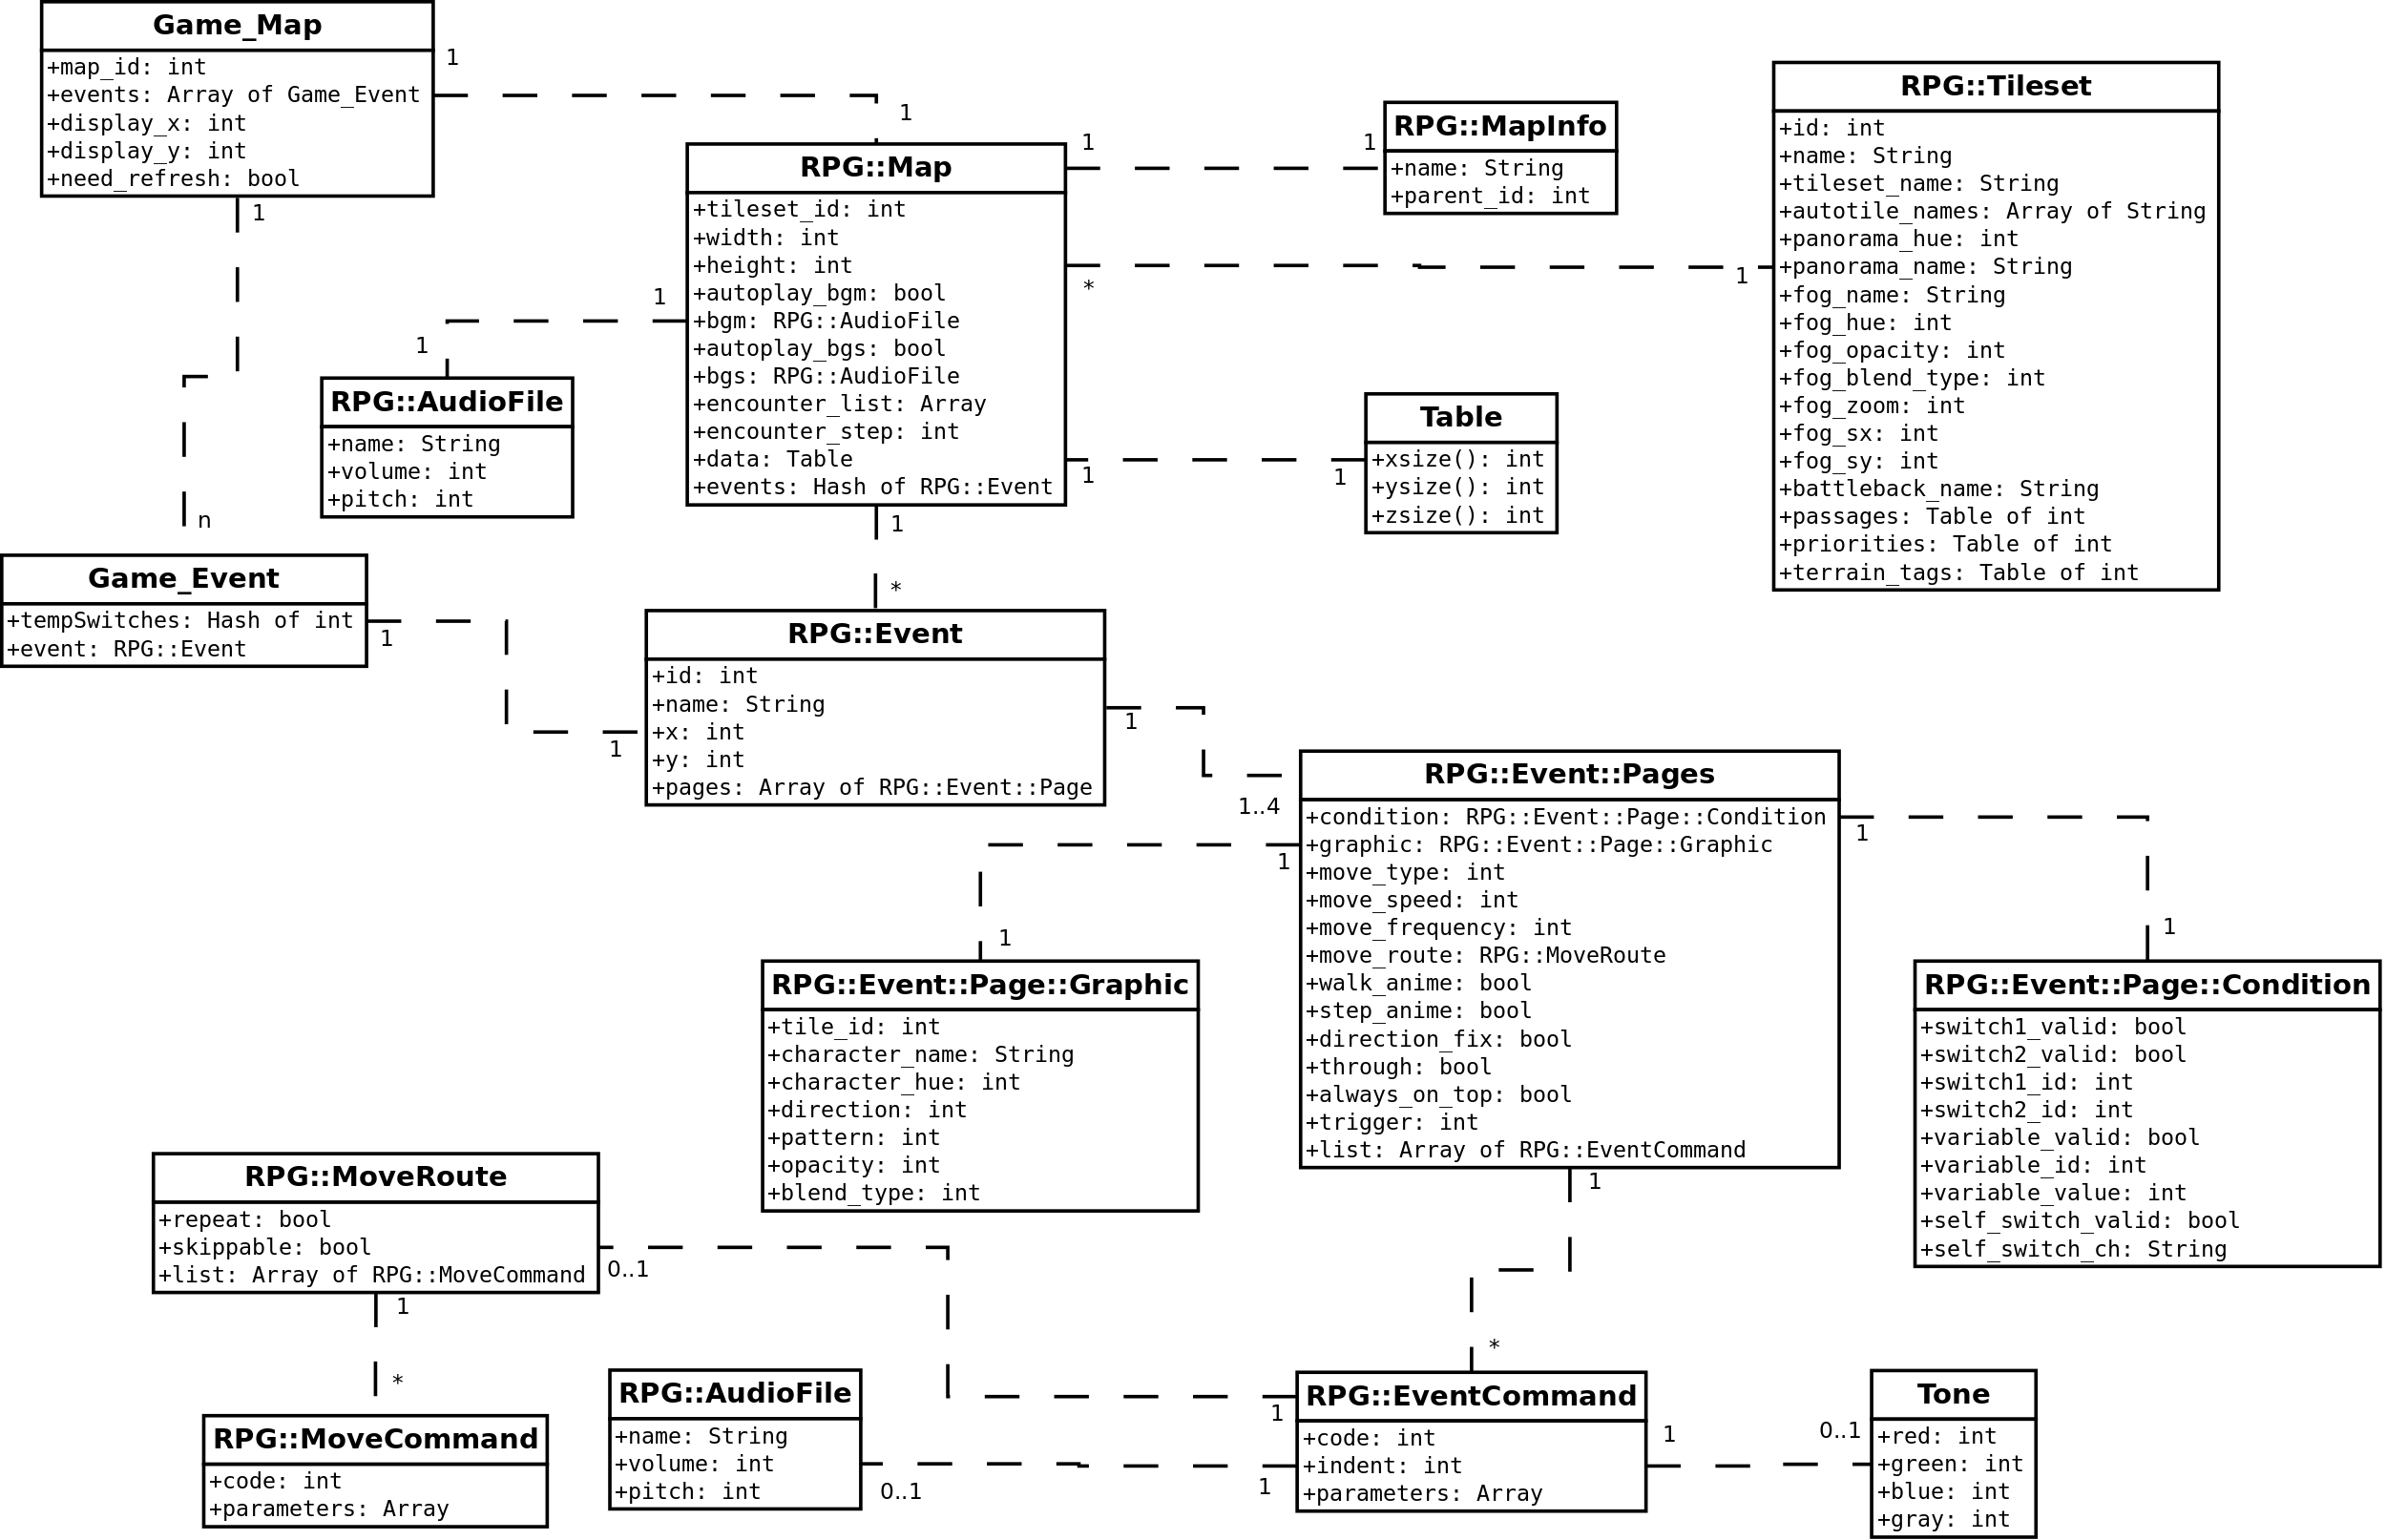
\includegraphics[width=\linewidth]{RMXP_full}
	\caption{Simplified class map representation for Map/Event}
	
\end{figure}


\textit{Semantic/Syntax} : Linked classes (with arity) display an \textbf{associative relationship}.

\textit{Note} : There is no inheritance relationship between any two classes represented. Arities are logically deduced and may not be exact depending in proprietary implementation details. Class \verb|RPG::AudioFile| was duplicated for ease of association routing.

Fortunately, only a subset of the information contained in this diagram is absolutely necessary and effectively extracted as map and event objects. Some can be abstracted or simply aren't used by Pokémon Essentials. 


\subsection*{Dialogue}

English dialogue is hard-coded in events, therefore in order to propose alternative languages, derived games must implement their own dialogue translation system. More research is needed on that front.

\newpage
\subsection{Data extraction process overwiew}
\begin{wrapfigure}[36]{l}{0.39\textwidth}
	\begin{center}
		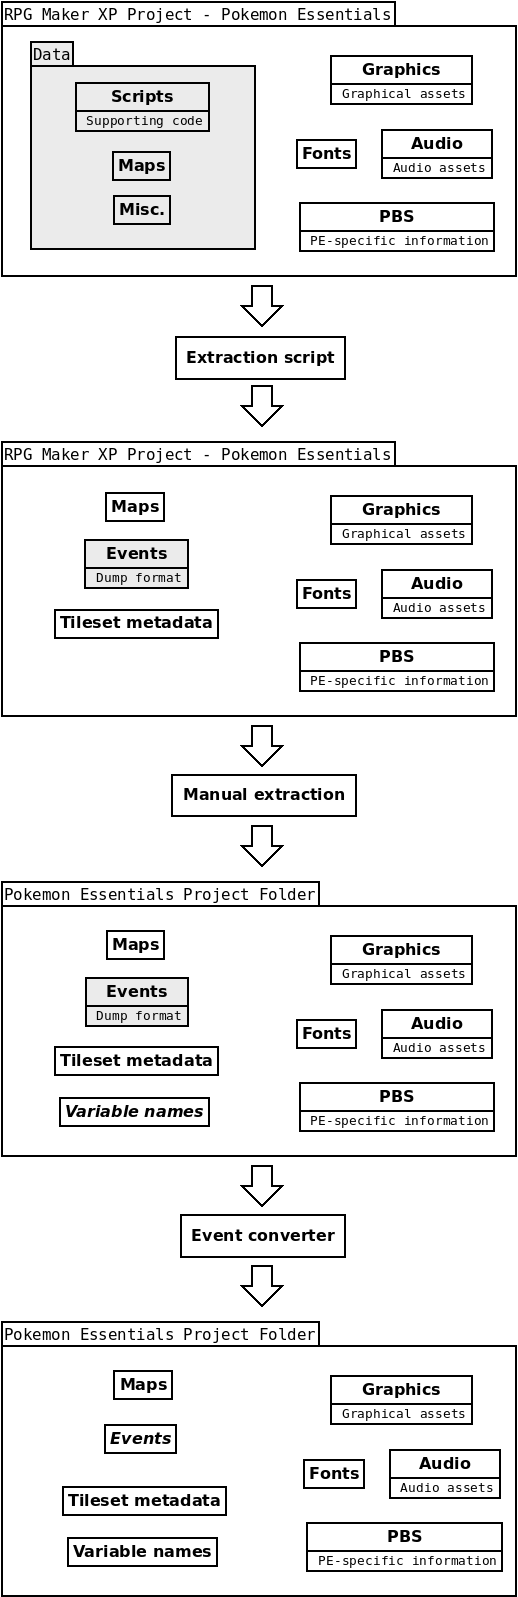
\includegraphics[width=1\linewidth]{Steps}
	\end{center}
	\caption{Extraction workflow}
\end{wrapfigure}


Pokemon Essentials, and other RPG Maker XP projects, have a clearly defined and standardized structure. Assets and data that make the content and logic of the game come in various formats, but for PoGER's purpose there is one important distinction :

\begin{itemize}
	\item Readily accessible data : Represented with white background, they exist in a standard format that can be interpreted/read without using RPG Maker XP.
	
	\item Obfuscated data : Represented with gray background, they are typically compiled and need the RPG Maker XP engine to interpret them.
\end{itemize}

PoGER's extraction effort aims to retrieve \textit{obfuscated data} and give it a standardized representation for use outside RPG Maker XP.

\vspace{2mm}
\textbf{Extraction script}

This script needs to be integrated to the game and executed. It does most of the heavy lifting, extracting \textbf{Maps}, \textbf{Events} (though only dumps them for further processing) and \textbf{Tileset metadata}.

\vspace{2mm}
\textbf{Manual extraction}

Unfortunately, no other way of retrieving the names associated with in-game variables and switches was found. They are needed because working with variable names is easier than with integer IDs.

\vspace{2mm}
\textbf{Event converter}

Events are surprisingly complex elements in RPG Maker XP, and the need for a new representation drove the development of an utility dedicated to that process.

Events are converted to a \textbf{domain-specific language} and packaged into individual easily editable files.

\vspace{2mm}
\textbf{Final result}

At the end of the extraction process, all assets and data used by the game exist in a RPG Maker XP-independent form.

This means that it's now possible for a third-party interpreter to run the game just like it ran on RPG Maker XP's!

\subsection{Automated extraction process}

Unfortunately, the first steps require the use of RPG Maker XP (version 1.02 tested, other should work also), and therefore Microsoft Windows (XP-10). It may be possible to run RPG Maker XP on other operating systems using a compatibility layer (such as Wine for GNU/Linux).


\subsubsection{Opening a project with RPG Maker XP}

Requirements : A copy of the project to extract. It should have the same structure as described in \verb|section 4.1.1|. Also, as previously mentioned, you need RPG Maker XP.

The following information was obtained through a trial-and-error process when trying to open the Pokemon Essentials and a derivative game (Pokemon Uranium) in RPG Maker XP and execute them in order to extract data from them. As such, they may contain erroneous statements or not apply/work for someone else trying to replicate the same process.

The following points should help you successfully opening a RPG Maker XP/Pokémon Essentials project :

\begin{itemize}
	\item You need the following files in the root directory :
	
	\begin{itemize}
		\item \verb|Game.exe| : The executable that launches the game.
		\item \verb|Game.ini| : A configuration file. If the \verb|*.ini| in the project has an other name, \textit{rename a copy} and \textbf{leave the original untouched}, because it seems RPG Maker XP needs a \verb|Game.ini| file and game can specify an other name (hard coded in scripts)
		\item \verb|Game.rxproj| : Entry point for RPG Maker XP.
		\item \verb|RGSS102E.dll| : Contain RGSS dynamic libraries, probably necessary tu run the executable correctly.
	\end{itemize}
	
	\item For projects with \textit{compressed data} (no \verb|Data| directory but there is one \verb|*.rgssad| file at root), you need to use an extraction utility.
	
	I used \texttt{RGSS Tool}\footnote{https://gitlab.com/rgss/rgsstool} :
	
	\begin{lstlisting}
	python rgsstool.py -x -d "path\for\output\files" "path\of\rgssad\file"\end{lstlisting}
	\vspace{-8mm}
	
	This worked with Python 3.x, google search it if you're not sure if you have a recent version of Python and how to launch it on your computer.
	
	Exemple for Pokemon Uranium when command line is at root :
	
	\begin{lstlisting}
	python rgsstool.py -x -d . Uranium.rgssad\end{lstlisting}
	\vspace{-6mm}
	
	\item For projects missing the \verb|Game.rxproj| file, simply create a new empty file and write the following: 
	
	\fbox{\ttfamily RPGXP 1.02}
	
	Save it with UTF-8 encoding and no "new line" character.
\end{itemize}

\newpage 
Tips :
\begin{itemize}
	\item Save files should be located in \verb|C:\Users\<user_name>\Saved Games\<name_of_the_game>\|
	
	\item When running the project from RPG Maker XP, some files in the \verb|Data| directory may be recompiled, which can cause errors. Keep a copy of the content of this directory in case you need to restore its content (you can exclude the \verb|Scripts.rxdata| if you're editing the scripts, so you don't lose progress on this file).
\end{itemize}
\hfill

\subsubsection{Executing the extraction script}

The role of the handcrafted script is to dump information accessible at runtime, some of which will need further processing to give it a useful representation.

Steps :
\begin{enumerate}
	\item Open the project in RPG Maker XP. Make sure the game can be launched (press \verb|F12| or click on the arrow next to the note icon).
	
	\item Open the script editor.
	
	\item Open \verb|Extraction.rb| and copy-paste its content to a new page in the script editor.
	
	\item Next step is tricky : You need to call the script from somewhere during execution. 
	
	\textbf{Recommended way} : Run the game within RPG Maker XP and play until you can gain control of the character and save. Close the game. Then, create an event close to your character and add a script command with parameter \fbox{{\ttfamily pbSaveAll()}}. 
	
	\textit{"Fast" (theoretical, untested) way} : Find the initial event that runs when the game launches and add to it a script command with parameter \fbox{{\ttfamily pbSaveAll()}}.
	
	\item Now, Launch the game again and trigger the event.
\end{enumerate}

Tip : Add "show text" commands before and after the script call to better visualize its execution (ex: "\textit{Click to save data.}" and "\textit{Done !}"). Also, you should be able to see the name of the window changing rapidly : it shows progress of the extraction process.

It works for Pokemon Essentials but may not work for its derivative works, especially if they changed data representations (unlikely) or if they contain unexpected data (likely).

After running the script, a few new folders should have appeared :
\begin{itemize}
	\item \verb|Maps| : Contain 2 files for each map (one for the map itself, the other for its events) and mirror the tree structure of the original project.
	\item \verb|Tileset_data| : Contain one file per tileset/autotile, storing metadata.
\end{itemize}

There should also be an \verb|Extraction.log| file, used to help debug issues with the script.


\newpage

\subsection{Manual extraction}

Unfortunately, we found some elements of RPG Maker XP to not be accessible using scripting or external utilities, thus making it impossible to automatically extract. Fortunately, they are scarce and easy to manually obtain from the UI.

\subsubsection{Switch and Variable names}

There are around 34 switches and a dozen variables used by Pokémon Essentials. They are used to store long-term information that are typically not specific to a particular event. Commands using them use their \textit{id} as reference, not their name.

While it is not strictly necessary to extract their corresponding names, it makes resulting commands way easier to read. The most straightforward id-to-name conversion strategy is to create a Python dictionary with ids as key and name as values. This allows conversion with a simple dictionary call.

You can find such an implementation in the \verb|PE_variables_switches.py| file.

Procedure to extract names :
\begin{enumerate}
	\item Create/Select an event, to display the "Event" window.
	
	\item Create a new event command. In the "Event command" window, select "Conditional Branch". \textit{There are other commands that could do the trick, we just chose this one}.
	
	\item On the "Conditional Branch" window, select either "Switch" or "Variable" and click on the switch/variable selection box immediately to its right.
	
	\item You should see a new window lists of items. Just select them one by one and copy-paste their name in the dictionary you're building (at the corresponding index of course).
\end{enumerate}


\subsection{Event processing}

Unfortunately, event porting is particularly complex for multiple reasons, including but not limited to :
\begin{itemize}
	\item The extracted objects are representations of RPG Maker XP's event interface, therefore inherits its structure additionally to useful information.
	
	\item The bulk of the behavior is expressed as event commands, which are numerous and need individual attention.
	
	\item The goal is to extract semantics into a new domain-specific language.
\end{itemize}

For this reason, a Python program was written for the purpose of processing the JSON-formatted event files from the previous step into usable files.








\newpage 
\section{Redefining Events}

\subsection{How RPG Maker XP stores data}

A crucial first step in any reverse-engineering effort in data extraction is to understand used data structures. As RPG Maker XP games run on a \textit{Ruby interpreter}, every element we encounter is either of a \textit{primitive type} or an \textit{object} (class instance).

Ruby primitive types :
\begin{itemize}
	\item Arrays
	\item Hashes
	\item Boolean
	\item Symbols
	\item Numbers
	\item Strings
	
\end{itemize}

\vspace{2mm}
For classes associated with maps and events, most of which are part of the RPG Maker XP library (other are defined in Pokémon Essentials scripts), see \texttt{Figure 2}.

\subsection{Events}

An event, or more precisely a \textit{map event}, is a way to introduce elements with behavior, therefore bringing flexibility and dynamism into the game world. Events have two representations :

%\vspace{2mm}
\begin{figure}[!h]
	\centering
	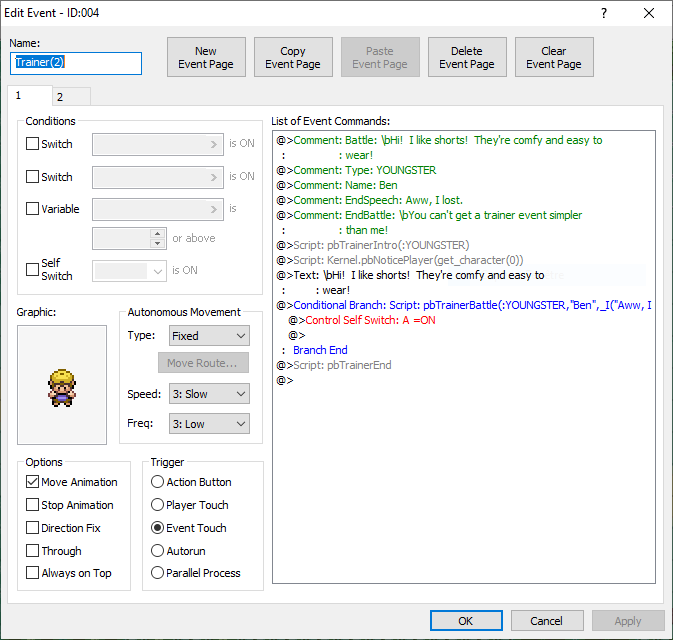
\includegraphics[width=0.63\textwidth]{Event} 
	\caption{How an event looks like using RPG Maker XP's GUI }
	
\end{figure}

\newpage
\begin{figure}[!h]
	\centering
	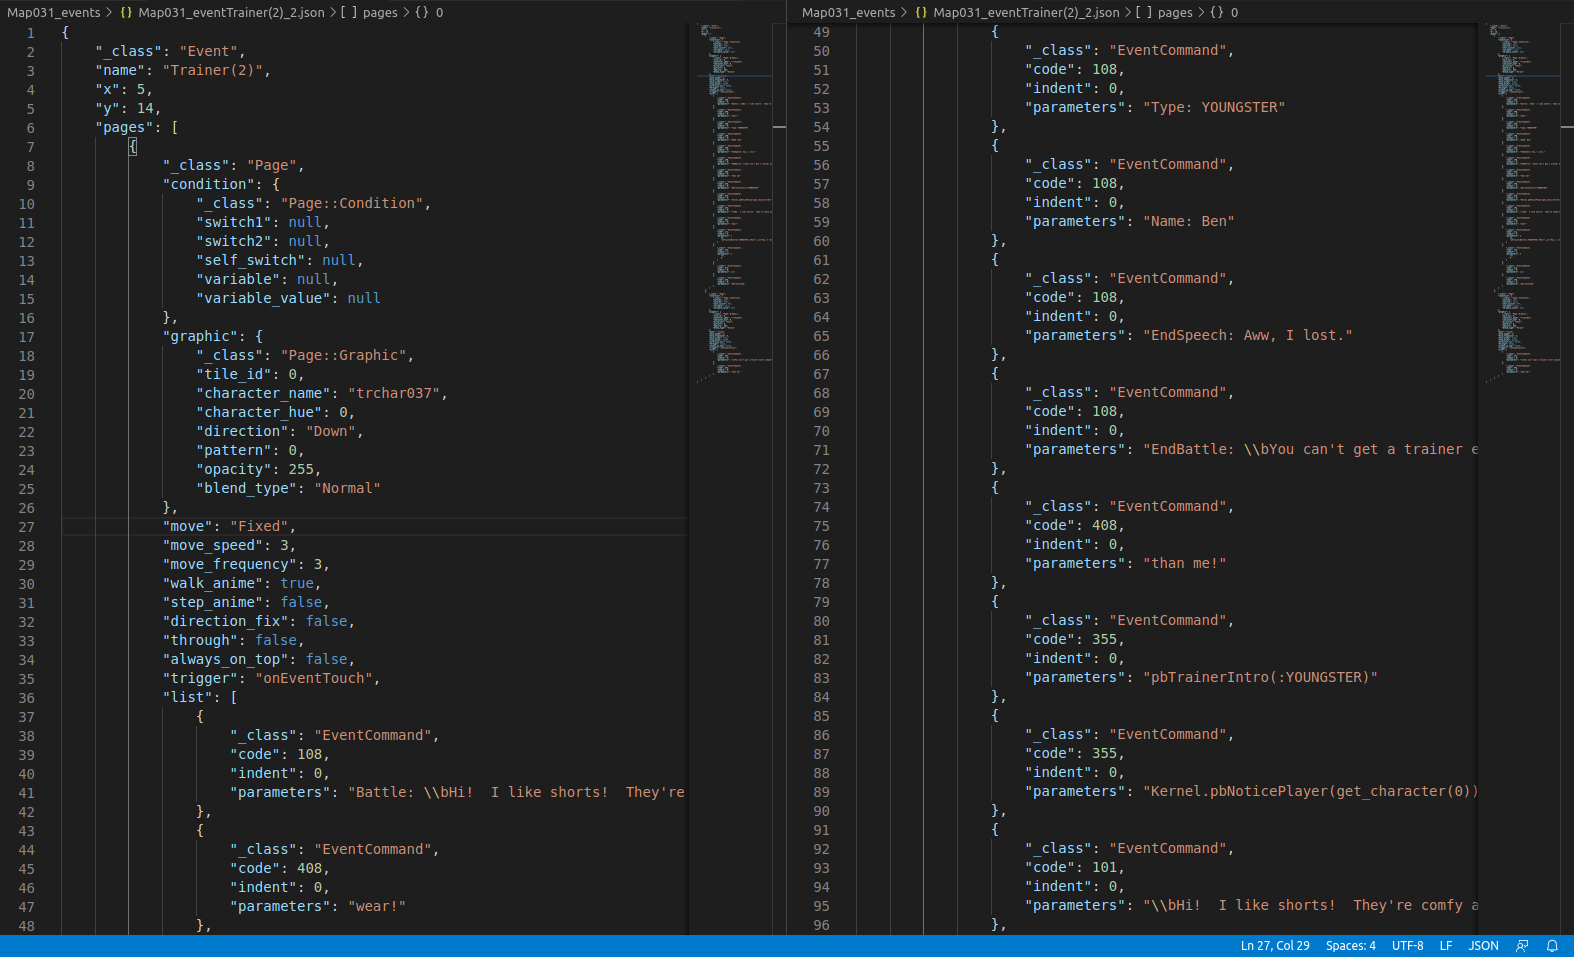
\includegraphics[width=\textwidth]{Event_json}
	\caption{Its data class instance counterpart \texttt{RPG::Event}}
	
\end{figure}


Events are highly complex objects, providing game makers with ample amounts of customization and tweaks to create any dynamic map element they may need. The following sections will explore functionalities, with a focus on the ones used by Pokémon Essentials.




\subsubsection{Basic functionalities}

These are the easiest and most straightforward behavior to implement into an event :

\begin{itemize}
	\item Giving an element a \textit{sprite} (texture) : This is useful for objects capable of movement, NPCs, etc.
	
	\item \textit{Movement} : Select how the element moves with presets (speed, frequency, pattern, etc).
	
	\item \textit{Event commands} : Select the trigger for behavior and what the element does when triggered (movement, dialogue, etc) within the extensive command list.
\end{itemize}

\subsubsection{Advanced functionalities}

These require an understanding of conditional execution and scripting :

\begin{itemize}
	\item \textit{Conditional execution} : branching instructions based on the value of : global variables, global switches, self switches, script return, etc.
	
	\item \textit{Pages} : Allow to give an element different behavior depending on conditions.
	
	\item \textit{Move routes} : Define a sequence of movement commands to be executed.
	
	\item \textit{Script calls} : Call a script to be executed for more complex behavior, launching mini-games, retrieving data, etc.
\end{itemize}

Script calls are particularly powerful because it allows arbitrary code execution. In simple terms, it enables events to do almost anything, providing it can be done through RGSS scripts.

As seen in \texttt{Figure 2}, every event can have up to 4 pages, and each page can have an arbitrary number of \texttt{EventCommand}s. Once the event is triggered, the appropriate page's command list will be executed.

The page decision goes as follows : Each page's preconditions are evaluated, and the latest page with satisfied preconditions is executed. We found that a tacit rule is that the first page typically has no precondition, effectively making it the "default" behavior and avoiding game crashes caused by an inability to trigger events successfully.



\subsection{Commands}

Commands are a mechanism, through which most of an \verb|RPG::Event|'s behavior is defined. Although they are very similar in structure and use, a distinction is made between \verb|RPG::EventCommand| and \verb|RPG::MoveCommand|.

\textit{EventCommands} are the representation of elements present in the "List of Event Commands" in the GUI. They are the building block of event's behavior.

\textit{MoveCommands} are the representation of an individual movement the event is capable of, typically found in sequences \verb|RPG::MoveRoute| associated with a dedicated \textit{EventCommand}.

They both have, at least :
\begin{itemize}
	\item A \textit{code} : An integer that uniquely identifies the particular command.
	\item \textit{Parameters} : Depend on the particular command, can be empty, a variable, an object, or a list of objects.
\end{itemize}

Additionally, \textit{EventCommands} have an \textit{indent} integer value, tied to the layout visible in the "List of Event Commands" in the GUI.




\subsubsection{Methodology}

In order to successfully \textit{extract semantic from events}, it was decided that \textit{documenting} every command used in Pokemon Essentials and finding an appropriate (human-readable) \textit{representation} was the way forward.

The objective is to formalize a \textbf{DSL} (Domain Specific Language) into which events will be translated to, which exhibit desirable properties.


For the sake of brevity, a lot of content was moved to \textbf{Appendix A}, mainly detailed information about each command used by Pokémon Essential events.



\newpage
\subsection{Command Representation}

The representation chosen is a result of careful consideration of its future usage requirements, including but not limited to :

\textbf{Readability} : It is destined to be read and written by humans, therefore it should be as straightforward and non-cryptic as possible.

\textbf{Brevity} : In the interest of anyone (human or software) reading/writing it, the \textit{less is more} approach is to be applied : instructions should not be longer than what is necessary.

\textbf{Unambiguity} : As any formal language, its use and syntax should be unambiguous.

\textbf{Simplicity} : Limiting the amount of available instructions by combining related ones is good practice.

\textbf{Expandability} : There should be room left for additional behavior to be implemented.



\subsubsection{Particular decisions}


\textbf{Python syntax style} : Reduces explicit syntax (like semicolons and curly braces), therefore reducing syntax error opportunities. Takes advantage of "implicit" syntax by making indentation itself meaningful.

\textbf{Case insensitive} : Simplification allowing any program to simply make everything lowercase when reading an \textit{Event}, and game makers to use any casing style they prefer. This also makes it harder to have variable/switch name collisions by forcing users to explicitly name their variables. An exception is made for double quoted strings, which typically contain text to be displayed and should be excluded (its format should be preserved).

\textbf{Switches, self-switches and variables} : Should be all represented as \textbf{symbols}. 

Proposed representation : \verb|":s" [String]| \textit{(string beginning with colon)}

Let \verb|s| be the string representation (name) of the Switch/Self-switch/Variable. \verb|s| of length 1 is to be reserved to self-switches.


\textbf{Ideas}
\begin{itemize}
	\item Timers could be implemented as integers : Let \verb|:PlayTime| be a read-olny integer variable that counts the seconds of play time (an \texttt{epoch}\footnote{https://en.wikipedia.org/wiki/Epoch\_(computing)} of sorts).
	
	Then, setting a timer for $x$ seconds could be as simple as storing (\verb|:PlayTime| + $x$) in a variable and testing it later against the current value of \verb|:PlayTime| !
	
	\item Commands have parameters (see examples) :
	\begin{itemize}
		\item No parameter : command line must contain the command keyword only.
		\item 1 parameter : command line must contain the command keyword, plus the expected parameter \verb|parameter_name = parameter_value| (parameter name recommended but not mandatory; parameter may be facultative)
		\item n$>$1 parameters : command line must contain the command keyword, and the expected parameters \verb|parameter_name = parameter_value| as a comma-separated list (no brackets; parameter name mandatory; parameter may be facultative).
		\item Note on \textit{facultative} parameters : marked with a \verb|*|.
		\item Strictly equivalent : '\verb|:ON|'$\equiv$'\verb|True|', '\verb|:OFF|'$\equiv$'\verb|False|', '\verb|is|'$\equiv$'\verb|==|' (when placed where a comparator would be).
	\end{itemize}
\end{itemize}


\subsection{Proposed command representation}

In an attempt to implement a Domain Specific Language (DSL) responding to previously stated requirements, a command list and formal grammar were included in \textbf{Appendix B} and \textbf{Appendix C} respectively.

\newpage
\subsubsection{Configuration variables}

These configuration variables are inherited from RPG Maker XP's events. They should be mostly contained at the root of the event, but can be overridden by the pages.

\begin{table}[!h]
	\centering
	{\footnotesize 
		\begin{tabular}{|a|c|c|l|}
			\hline
			\textbf{CONFIG\_VAR} & \textbf{type} & \textbf{Default} & \textbf{Description}. \\
			\hline
			{\ttfamily name} & {\ttfamily String} & N/A & Identifies the event. \\
			\hline
			{\ttfamily xy} & {\ttfamily [int, int]} & N/A$^*$ & Position of the event. \\
			\hline
			{\ttfamily graphic} & {\ttfamily String/int} & None & Texture of the event. \\
			\hline
			{\ttfamily pattern} & {\ttfamily int} & 0 & Column index for the sub-texture from \verb|graphic| to use. \\
			\hline
			{\ttfamily opacity} & {\ttfamily int} & 255 & \verb|0-255| Opacity for event's texture. \\
			\hline
			{\ttfamily transparent} & {\ttfamily bool} & False & Transparency flag. When enabled, \verb|graphic| isn't displayed. \\
			\hline
			{\ttfamily direction} & {\ttfamily String} & S & [N,E,S,W] Initial facing direction (if has {\ttfamily graphic}). \\
			\hline
			{\ttfamily trigger} & {\ttfamily String} & "onPlayerAction" & Trigger for the behavior of the event. \\
			\hline
			{\ttfamily move\_animation} & {\ttfamily bool} & True & Whether the graphic should be animated when moving/walking. \\
			\hline
			{\ttfamily stop\_animation} & {\ttfamily bool} & False & Whether the graphic should be animated when not moving/walking. \\
			\hline
			{\ttfamily direction\_fix} & {\ttfamily bool} & False & The direction (of the texture) of the event cannot be changed \\
			&  &  & when True. \\
			\hline
			{\ttfamily through} & {\ttfamily bool} & False & "Walk through walls" switch: when True, collision is ignored and \\
			&  &  & the event can go anywhere (walk on water, walls, holes, etc). \\
			\hline
			{\ttfamily always\_on\_top} & {\ttfamily bool} & False & Event's graphic should be drawn last, as to always be "on top" \\
			&  &  & of everything else. Scarcely used. \\
			\hline
			{\ttfamily movement} & {\ttfamily String} & "Fixed" & "Fixed", "Random" or "Approach". \\
			\hline
			{\ttfamily movement\_speed} & {\ttfamily String} & "Slow" & "Slow" or "Fast". Vaguely defined. Player's movement is "Fast". \\
			\hline
			{\ttfamily preset} & {\ttfamily String} & None & Proposed "preset" for simple, common events (boulder, door, etc). \\
			\hline
		\end{tabular}
	}
	\caption*{$^*$ : Mandatory configuration, therefore no default.}
\end{table}

Notes :
\begin{itemize}
	\item \verb|graphic| can be either a string (name of a character file) or an int (\textit{tile id} from the current tileset). Defaults to None : the event has no texture.
	
	\item \verb|move_animation:False, stop_animation:True| is mostly used for berry trees.
	
	\item \verb|trigger| can have values : 
	\begin{itemize}
		\item \textit{onPlayerAction} : The event is triggered by the player interacting (using action button) with it.
		
		\item \textit{onPlayerTouch} : The event is triggered by the player touching (walking into) it.
		
		\item \textit{onTouch} : The event is triggered by the player touching (walking into) it OR the event touching the player.
		
		\item \textit{onAutorun} : The event is triggered when the map is loaded.
		
		\item \textit{ready} : The event is always triggered, its execution is controlled through its behavior conditions.
		
		\item \textit{onSeen n} : The event is triggered when the player is on the event's line of sight, within n tiles (n is optional, defaults to no limit)
	\end{itemize}
	
\end{itemize}







\newpage
\subsection{Command conversion caveats} % Alliteration is fun !

Unfortunately, it is not possible to cover every command used in Pokémon Essentials, just as it is not possible to extract the underlying semantic behind every event, for the simple reason that Pokémon Essentials doesn't always implement behavior in a straightforward way.

Reading some events, it appears obvious that the authors of Pokémon Essentials had to work around limitations of event commands, relying on scripts to expand capabilities. These result in artifacts.

These include, but are not limited to :

\textbf{Recurring events} : Some events, like \textit{doors}, are common and have straightforward behavior, so authors just copy-pasted them everywhere they were needed, only applying modifications when necessary (eg: appearance and transfer destination on doors).

These were the motivation behind the creation of the \verb|preset| configuration variable on events. It would allow for all recurring commands to be abstracted away, allowing for shorter and cleaner events.

\textbf{Text hack} : According to Pokémon Essentials's wiki \cite{PEmessages}, there are plenty of modifiers that can be integrated to text in order to modify its behavior : changing text font, size, setting it bold, italic, changing its position or alignment, displaying a selection menu, etc..

This would need to be re-implemented entirely to replicate behavior.

\textbf{Arbitrary code} : The ability to execute scripts in events, and the globally accessible nature of most elements in the game, allows scripts to perform basically any action.

Replicating this much flexibility without a Ruby interpreter and Pokémon Essentials's original scripts would be completely impractical. The only sensible way forward would be to implement the basic function calls and elevate the abstraction level for complex behavior, or fixing it by hand. Decision are to be made on a case-by-case basis. Fortunately, only a few events require such attention.

\textbf{Arbitrary variable use} : This is not exactly an artifact or RPG Maker XP's limitations, but one of Pokémon Essentials's authors. They sometimes use variables,  whose name imply a certain usage scope, for unrelated purposes. 

This could have been simply avoided by creating new variables. It is not technically an issue : the game already runs with these artifacts, therefore it doesn't need fixing. There is no other solution than fixing it by hand (by creating new variables and changing usage).




\subsection{Event conversion software}

Subsection about contents of \texttt{Event converter} directory






\newpage 
\section{Event Interpreter}

% Pokémon Essentials Next interpreter

During the course of the extraction process, event's data was dumped and translated into the proposed Domain Specific Language. The last logical step would be to provide an interpreter capable of executing them, and that's what this section is about.

\subsection{Proof of concept}

You can find the files for this implementation in the \texttt{Interpreter} directory. It was coded in Python (version 3.x) but an equivalent program could be written in most popular languages.

The proposed interpreter can be decomposed in two parts. The first builds an \texttt{Event} object from its file, and the second executes it. Let's focus on the first part :

\begin{wrapfigure}[31]{l}{0.27\textwidth}
	\begin{center}
		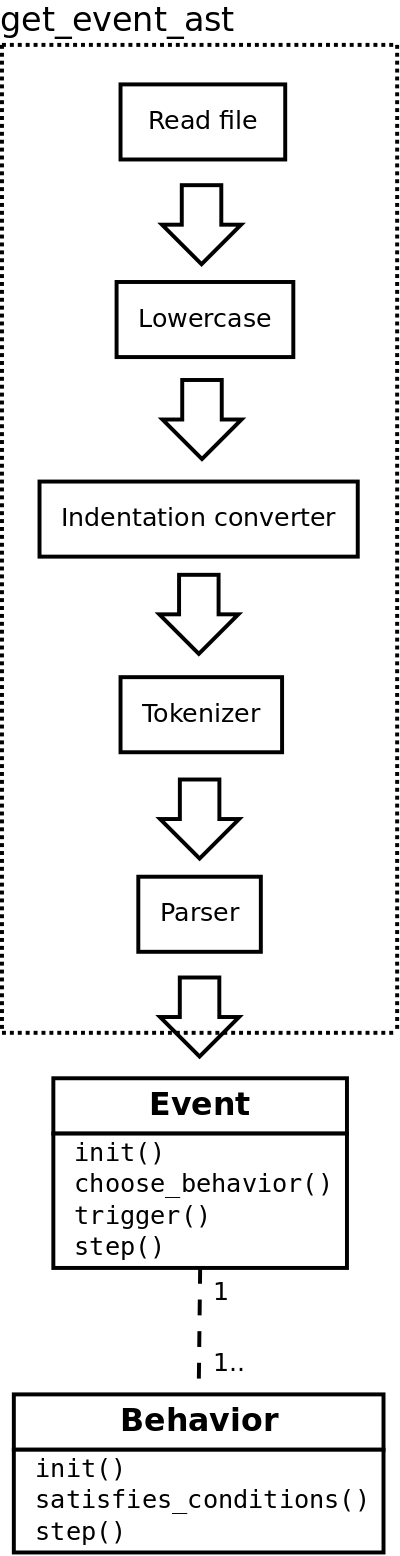
\includegraphics[width=.9\linewidth]{Interpreter}
	\end{center}
	\caption{Interpreter}
\end{wrapfigure}

\textbf{Flow diagram syntax} : Rectangles are data manipulation functions and big arrows represent the passage of said data.

\textbf{Read file} : The contents of the event file are read.

\textbf{Lowercase} : As discussed in previous sections, the DSL is case-insensitive. To simplify next steps, lowercase transformation is applied. Note that text between double quotes must be excluded, and that uppercase transformation could have been chosen instead.

\textbf{Indentation converter} : The DSL's specification indicate that indentation is significant. This step converts it because only relative indentation (from one line to the next) has semantic value and should be represented, and also because the tokenizer we used didn't produce intentation tokens.

\textbf{Tokenizer} : We used the tokenizer generator from \texttt{funcparserlib} \cite{funcparserlib} to generate a stream of tokens from a string (the data at the input of the tokenizer) and a list of rules. This lexer is particular because it was made to work with the parser of the same library, which we use for the next step !

\textbf{Parser} : We used the parser generator from \texttt{funcparserlib} \cite{funcparserlib} to generate an abstract syntax tree (AST) from the DSL's formal grammar.


\verb|get_event_ast| is called by an \texttt{Event} during its initialization process: from its file, it gets an AST representation from which it can easily reconstruct its configuration and behaviors. This allows the creation of events with a very simple interface !

This approach has a few key properties : Because the AST is generated from the DSL's formal grammar, its format is known in advance and it can be generically processed by \texttt{Event}s and its \texttt{Behavior}s, making it possible to expand the DSL without necessarily having to adapt  their implementation. Also, the event file may contain syntax or grammar errors. If so, the lexer or parser will raise an error with information to correct it.

\newpage
\subsection{Executing an event}

Once an \texttt{Event} object is correctly initialized, it may be triggered. This is done by calling its \texttt{trigger()} method with the trigger identifier, which is compared to the event's trigger (defined via configuration). If matched, the event is successfully triggered.

A triggered event will evaluate which behavior to execute based on the returned value of each associated \texttt{Behavior}'s method \texttt{satisfies\_conditions()}. See \texttt{Section 5.2.2} for details. 

Then, the event's \texttt{step()} method may be called for it to execute one "step" of its behavior. What instructions represent a "step" or not is a decision left to the interpreter, but the general rule is : Only the instructions that have an observable impact on the game world (displaying text, moving the event, playing a sound, waiting, etc) should end a step. Therefore, calling \texttt{step()} implies the execution of an arbitrary number of instructions.

Behavior execution is achieved by maintaining a representation of the instructions left to execute and passing it to the interpreter's \texttt{execute()} method, which takes care of executing instructions one by one and returning an updated "remaining instruction" object and whether the step is over or not.

The implementation strategy for the \texttt{Interpreter} is straightforward : It holds the state of the game (keeps track of global variables) and each instruction of the DSL has its own function which is called by the \texttt{execute()} method. This modular approach was chosen for its ease of maintainability and expandability.  See \texttt{Interpreter.py}

A secondary interpreter was created, with a very similar structure, but with the goal of enabling \textit{script interpretation}. As previously discussed, some events rely on RGSS script calls to implement part of their behavior, but writing a full RGSS interpreter would be too complicated. The envisioned solution was to re-implement these specific scripts in that interpreter, massively reducing its scope while keeping functionality intact. See \texttt{pbInterpreter.py}


\subsection{Current state of the interpreter}

For the moment, the event interpreter only exists as a "proof of concept" (POC), therefore is very basic and implements only a few instruction of the proposed DSL. It was made tested with basic handcrafted event files and Pokémon Essentials's \textit{Fossil reviver} (found at map 11, chosen because its behavior is neither too simple nor too complex), so the best it can do is a short demo.

With some more work, it could be made into a fully-featured interpreter capable of executing every event in Pokémon Essentials or a derived project. Such a piece of software would be a module of the PoGER project, which aims at running these games.



\newpage 
\section{RPG Maker XP Maps}

As stated previously, maps are instances of \verb|RPG::Map|, which constitutes the game world, describes its appearance and hosts its events. Here are its components :

{\small
\begin{tabular}{|a | l | l|}
	\hline
	{\ttfamily tileset\_id} & int & \parbox{.66\linewidth}{\vspace{.2\baselineskip}Value of a {\ttfamily RPG::Tileset} unique identifier component {\ttfamily id}. The {\ttfamily RPG::Tileset} object can be retrieved through the global hash {\ttfamily \$data\_tilesets} using the id as the key.} \\
	\hline
	{\ttfamily width,height} & int,int & Attribute equivalent to \verb|data.xsize()| and \verb|data.ysize()|. \\
	\hline
	{\ttfamily autoplay\_bgX} & bool & Indicated whether an audio is to be played as soon as the map is loaded. \\
	\hline
	{\ttfamily bgm/bgs} & AudioFile & The audio to be played when loading the map. \textit{bgs unused by PE} \\
	\hline
	{\ttfamily encounter\_list} & Array & \textit{Unused by Pokémon Essentials}. \\
	\hline
	{\ttfamily encounter\_step} & int & \textit{Unused by Pokémon Essentials}. \\
	\hline
	{\ttfamily data} & Table of int & Contain the \textit{map} representation of the 3 tile layers. \\
	\hline
	{\ttfamily events} & Hash & Contain the \textit{Event} representation ({\ttfamily RPG::Event}) for this map. \\
	\hline
\end{tabular}}

Crafting a map data representation for extraction (and further use) requires understanding the meaning of these components, the role of associated classes and the functioning of graphical assets. This is what this section explores.


\subsection{Associated classes}

In \texttt{Figure 2}, we can observe that instances of \verb|RPG::Map| have ties with instances of different classes:

\begin{itemize}
	
	\item About the associated \verb|RPG::MapInfo| instance : It contains a few useful informations :
	
	{\small
	\begin{tabular}{|a | l | l|}
		\hline
		{\ttfamily name} & String & The name of the map. \\
		\hline
		{\ttfamily parent\_id} & int & In the map tree, the id of the parent map. \\
		\hline
	\end{tabular}}
	
	This information can retrieved directly from the compiled \textit{MapInfos} file :
	\begin{lstlisting}[language=Ruby]
	mapinfos = pbLoadRxData("Data/MapInfos")
	map_name = mapinfos[id].name
	parent_map_id   = mapinfos[id].parent_id
	parent_map_name = mapinfos[parent_map_id].name rescue nil\end{lstlisting}
	\vspace{-8mm}
	RPG Maker XP allows maps to be structured in a hierarchy, where a map can have a "parent map". This information is used to replicate this property on extracted map data.
	
	\item \verb|RPG::Tileset| : Represents a normal tileset :

	{\small
	\begin{tabular}{|a | l | l|}
		\hline
		{\ttfamily id} & int & The id of the tileset. \\
		\hline
		{\ttfamily name} & String & Its name (no extension). \\
		\hline
		{\ttfamily tileset\_name} & String & Name of tileset. \textit{Moved to Map}. \\
		\hline
		{\ttfamily autotile\_names} & Array of String & Names of associated autotiles (up to 7). \textit{Moved to Map}. \\
		\hline
		{\ttfamily panorama\_*} &  & \textit{Unused by Pokémon Essentials}. \\
		\hline
		{\ttfamily fog\_*} &  & \textit{Unused by Pokémon Essentials}. \\
		\hline
		{\ttfamily battleback\_name} & String & Name of the texture that appears during combat. \textit{Moved to Map}. \\
		\hline
		{\ttfamily passages} & 2D Table of int & Properties of individual textures. \\
		\hline
		{\ttfamily priorities} & 2D Table of int & Properties of individual textures. \\
		\hline
		{\ttfamily terrain\_tags} & 2D Table of int & Properties of individual textures. \\
		\hline
	\end{tabular}}
	
	\item The role of the associated \verb|Game_Map| instance is to be studied further, but current understanding indicates that it's an alias derived from its \verb|RPG::Map| instance that is tailored for Pokémon Essentials's needs. Therefore, it holds no useful data and can be safely disregarded.
	
	
	\item \verb|RPG::AudioFile| : Basic data container :
	
	\begin{tabular}{|a | l | l|}
		\hline
		{\ttfamily name} & String & The name of the audio file (no extension). \\
		\hline
		{\ttfamily volume} & int & Acts like a volume slider, normalized at 100. \\
		\hline
		{\ttfamily pitch} & int & Allows to adjust sound pitch, normalized at 100. \\
		\hline
	\end{tabular}
	
	A global variable (\verb|$data_tilesets, Array|) stores this information.
	
	\item \verb|Table| : Used for 2D/3D arrays, with 3 class mathods to retrieve dimensions. $x$ and $y$ correspond to their GUI map representation and $z$ the map layers (background, intermediate, foreground).
	
\end{itemize}


\subsubsection{Values for tileset tables}

Each table contains \verb|int| values, one per texture for each category. This value is to be interpreted .

\verb|passages|: let's consider the 6 least significant bits
\begin{itemize}
	\item bit 0 : Can't come from S
	\item bit 1 : Can't come from W
	\item bit 2 : Can't come from E
	\item bit 3 : Can't come from N
	\item bit 4 : Is a bush
	\item bit 5 : Is a counter (tile through which interaction is possible)
\end{itemize}

Examples : a bush at which the player can come from any direction has value \verb|0b01 0000 = 16|, and an obstacle (which isn't a counter) has value \verb|0b00 1111 = 15|.

\verb|terrain_tags|: see \verb|PBTerrain| module for values. They are used by Pokémon Essentials, mostly to determine if an action is compatible with a tile (eg : surfing, diving, climbing, etc).


\verb|priorities|: default value is 0. Any higher value means that the texture has priority. In practice, it means that the texture is "above" its own layer (drawn last). Combined with passability, it's possible for it to be on the same layer as NPCs/the player and give the illusion that they can pass behind it. It's mostly used for the top of tall trees, houses, etc.

Proposition : integrate \verb|priorities| to \verb|passages| as a \nth{7} bit (\textit{bit 6 : Can be passed behind}). Note that this proposition is implemented in the extraction script.


\subsection{About graphical assets}

When dealing with (most) graphical assets in RPG Maker XP, including tilesets, autotiles and maps, a few constraints apply :

\begin{itemize}
	\item The base unit is the \textbf{tile}, which is a 32 by 32 square.
	
	\item Tilesets must have a horizontal dimension of exactly 8 tiles (256 pixels), but can be arbitrarily tall (n tiles tall).
	
	\item Tilesets can have up to 7 associated autotiles. This has proven to be a limiting factor in Pokémon Essentials.
	
	\item Autotiles are special assets. They can be put on a map like any texture from a tileset, but have the properties of being context-aware and animation-capable :
	
	They form coherent surfaces by manipulating components of their texture in order to give the impression of continuity when multiple instances of the same autotile are neighbors. They can be used to create basically any surface that needs to deal with how its border with an other surface looks.
	
	This property is generated at the moment of placing the autotiles by automatically determining the right index for each, and therefore is an artifact of the map editor.
	
	Two formats were identified (\textit{frames are situated side-by-side horizontally}) :
	\begin{itemize}
		\item $3N \times 4$ : a 3 tile horizontal, 4 tile vertical, $N$ frame image. This is the official autotile format for RPG Maker XP.
		
		\item $N \times 1$ : a 1 tile horizontal, 1 tile vertical, $N$ frame image. This is used for animated individual tiles.
	\end{itemize}

	Animation is produced by iterating over frames of an autotile each time the screen is drawn.
	
	\item Every tile has properties (see section "values for tileset tables"). This includes autotiles, which notably have a single \verb|passages|, \verb|terrain_tag| and \verb|priorities| value.
	
	\item During map reconstruction attempts, we found out that most maps only use a fraction of tiles available to them and programmed a way of converting maps and their tilesets to a "compact" format (creating an alternate tileset with only used tiles, and adapting map data accordingly).
	
	Although it is functional and may be advantageous for running on low memory systems, the scattering of graphical assets and the loss of tile adjacency render this approach pointless or impractical. 
\end{itemize}


We believe the decision of tying tiles and autotiles together in their object representation, and then using the original tileset file name to refer to said object in maps, was a poor design choice. In consequence, the extraction script decouples maps, autotiles and tilesets, allowing for more flexibility (for example, it raises the possibility of removing the 7 autotile per tileset limit).



\subsection{Autotile format}

Researching how autotiles are adaptively generated proved to be a tedious manual process of reverse-engineering. 

We used a "test map" we created as a starting point for studying Pokémon Essentials (included at \textbf{Appendix D}). By placing autotiles in various shapes and extracting map data, we were able to manually correlate tile content to their index (and understand both the absolute and relative indexing systems).

An article about the format of autotiles for another RPG Maker software \cite{Autotile} proved helpful for understanding how autotiles work. It turns out that autotiles tiles are divided into four separate "sub-tiles" of 16 by 16 pixels, and each index correspond to a combination of sub-tiles into a unique tile.

\vspace{4mm}
\begin{figure}[!h]
	\centering
	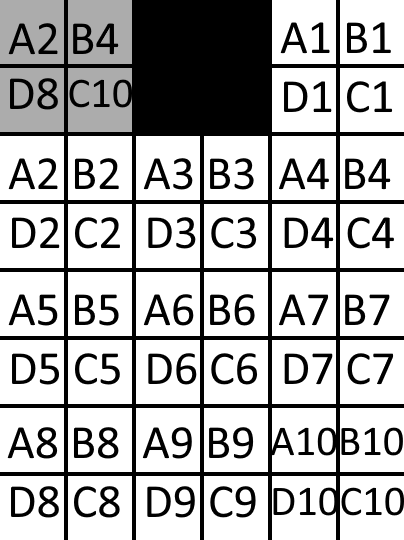
\includegraphics[width=.3\linewidth]{Autotiles_16x16}
	\caption{3 by 4, single frame autotile format}
\end{figure}
\vspace{4mm}

As you can see, only 10 tiles are actually used out of 12. Some autotile assets for Pokémon Essentials contained texture for the redundant/unused tiles for some unidentified reason, which make us suspect there might be something we are missing about their format.

The result of our research can be found in the \verb|AutotilesSubtileMap.ods| spreadsheet file. It lists indexes and their corresponding subtile components. A Python implementation (\verb|LoadImage.py|) is also provided : it can reconstructs maps from map data, tileset and autotiles, including GIF output (see \verb|Map032_out.gif| for example), demonstrating the feasibility of lossless map extraction and reconstruction.




\subsection{Map representation}

At its core, a RPG Make XP map is a \textit{tiled map} : it is a 2-dimensional grid of textures (tiles) of fixed size.

The \verb|data| component is a 3-dimensional table of integer values with the following properties :
\begin{itemize}
	\item The \nth{3} dimension is used to represent \textbf{layers} : exactly 3 tiled maps are used for any RPG Maker XP map :
	\begin{itemize}
		\item Background : Contains mainly the textures that make the ground and other elements that are always "below player's level". Any event or texture of higher layer will be displayed \textit{above} it.
		
		\item Intermediate : Contains mainly the textures that should be "at player's level", which includes most elements the player can interact with (including bumping into).
		
		\item Foreground : Contains mainly the textures that should be "above player's level", typically used for elements below which the player can stand.
	\end{itemize}
	
	\newpage
	\item Each layer obeys the same indexing convention :
	
	\begin{tabular}{|c|l|}
		\hline
		\rowcolor{mylightgray}
		\textbf{Value(s)} & \textbf{Description} \\
		\hline
		\verb|0| & Reserved value for "No texture" \\
		\hline
		\verb|1-47| & Reserved, unused. \\
		\hline
		\verb|48-95| & Range used for autotile 1. \\
		\hline
		\verb|96-143| & Range used for autotile 2. \\
		\hline
		$\vdots$ & \phantom{hi reader :wink:}$\vdots$ \\
		\hline
		\verb|336-383| & Range used for autotile 7. \\
		\hline
		\verb|384-| & Range used for tileset. \\
		\hline
	\end{tabular}
	
	This way of reserving 48 indexes per autotile results from autotile's mechanism for generating context-aware textures.
	
	Note : each range describes the \textit{absolute positions} between which a \textit{relative indexing system} takes place. For example, index 52 is interpreted as index 4 for autotile 1 and index 484 is index 100 on the tileset (remember that indexes begin at zero, not one).
	
\end{itemize}

With this information, a map can be reconstructed from indexes by mapping them to the corresponding textures and drawing the layers in order.




\subsection{Map and Tileset files}

There should be a well-defined way of representing extracted map and tileset information. 

\textbf{Map}
\begin{itemize}
	
	\item Located in the "\verb|Maps|" directory.
	
	\item Naming convention : \verb|<id>_<name>.json |. The \textit{name} is only here as a quality-of-life addition, for developers to easily know what map they're dealing with. It must be present, though.
	
	The extension isn't really important but reflects the content's format.
	
	\item Location agnostic : A map file can be at the root of the "Maps" directory, or in any subdirectory, allowing for the same flexibility as RPG Maker XP's UI.
	
	
	\item Content : utf-8 encoded JSON with the following entries
	
	{\small
		\begin{tabular}{|a | l | l|}
			\hline
			{\ttfamily \_class} & String & Must be \verb|"Map"|. \\
			\hline
			{\ttfamily name} & String & Map's name. Used for displaying current location. \\
			\hline
			{\ttfamily width} & int & Map's width. Should be checked against the content of {\ttfamily table}. \\
			\hline
			{\ttfamily height} & int & Map's height. Should be checked against the content of {\ttfamily table}. \\
			\hline
			{\ttfamily battleback} & String & Picture to be displayed behind battles. \\
			\hline
			{\ttfamily tileset} & String & Map's tileset (file name without extension). \\
			\hline
			{\ttfamily autotiles} & Array of String & Map's autotiles (file name without extension). \\
			\hline
			{\ttfamily autoplay\_bgm} & bool & Sets whether the bmg should be played when entering the map. \\
			\hline
			{\ttfamily bgm} & String & Map's background music.  \\
			\hline
			{\ttfamily table} & 3D array of int & Describes map's texture placement (3 layers).  \\
			\hline
	\end{tabular}}
	
	Note : \verb|bgm| formats : \verb|"<name>"| or \verb|"<name>,<volume>,<pitch>"|
	
	Note : \verb|table| must have dimensions \verb|width x height x 3|
\end{itemize} 

\textbf{Tileset and Autotiles}
\begin{itemize}
	
	\item Located in the "\verb|Tileset_data\Tilesets|" and "\verb|Tileset_data\Autotiles|" directories respectively.
	
	\item Naming convention : \verb|<name>.json |. The \textit{name} is only here as a quality-of-life addition, for developers to easily know what map they're dealing with. It must be present, though.
	
	
	\item Content : JSON with the following entries
	
	{\small
		\begin{tabular}{|a | l | l|}
			\hline
			{\ttfamily \_class} & String & Must be \verb|"Tileset"|. \\
			\hline
			{\ttfamily name} & String & Tileset's file name (no extension). Referenced by map's property \verb|tileset| \\
			\hline
			{\ttfamily passages} & (1D array of) int & Tileset's passage table. \\
			\hline
			{\ttfamily terrain\_tags} & (1D array of) int & Tileset's terrain tag table. \\
			\hline
	\end{tabular}}
	
	Note : for autotiles, all values in \verb|passages| and \verb|terrain_tags|, therefore these fields were simplified to a \textit{single integer value}.
	
	Note : RPG Maker XP seem to fail to load tilesets/autotiles after an extraction with destination "\verb|Graphics\Tilesets|" and "\verb|Graphics\Autotiles|" directories, probably because there are foreign files in the graphic folder. For that reason, other directories were used.
	
	\item Advantages : Decoupling a \verb|Tileset| from the autotilesets used for a particular map allows added flexibility.
\end{itemize}

\newpage
\subsubsection{On naming decisions}

We were asked about the use of a 3-digit numerical identifier in the file names, and why we didn't choose to use name identifiers instead. Numerous considerations ensued :
\begin{itemize}
	\item First of all, numerical identification was originally used for maps, tilesets, etc
	
	Therefore, transitioning to another identification system would be complex and an exercise in reinventing the wheel, all that for questionable gain.
	
	\item Using a file name identifier means that identification information needs to reside inside the file itself due to restriction on file name contents imposed by various file systems.
	
	Without it being in the name, some other strategy of file identification would be needed :
	\begin{itemize}
		\item Reading each file, looking for the one containing the right id
		\item A database associating each file with its id
	\end{itemize}
	None of these are particularly engaging.
	
	\item The idea of using names for identification is attractive at first glance : user-friendly and intuitive, it's great !
	
	Unfortunately, there are some issues with this solution, including but not limited to :
	\begin{itemize}
		\item As stated before, it would be complex to transition to this new identification system.
		
		\item Not all characters are usable : every file system imposes limitations, which would impose unwanted restrictions for developers.
		
		\item Dealing with names/strings means that ids are typically longer and less formally defined (can contain more caracters, including casing, accents, etc), therefore amplifying the risk of any id containing errors.
		
		
		\item Developers involved in this type of project are typically capable of dealing with numerical ids without issue already.
		
		\item For large projects with hundreds/thousands of maps, name collisions may force developers to use convoluted or cumbersome naming schemes.
	\end{itemize}
	
	Note that some of the issues identified may be circumvented by re-introducing the "name" field in the files themselves, but at this point the percieved value of the change would become nil.
	
	\item While it is true that numerical id collisions is possible and using name ids may help preventing them, there are other strategies available. 
	
	Planning, for example : reserving ranges of values for specific uses ahead of time.
\end{itemize}

\vspace{4mm}
In conclusion, it is our estimation that using numerical ids is a reasonable choice, as it is a tried-and-true solution that doesn't compromise on usability (at least not too much).

On the other hand, the suggestion of abandoning the 3 digit format for numerical ids was considered and adopted, as it would allow larger projects to exist and didn't pose any technical problem.

\newpage
\subsection{Map reconstruction}


Subsection about contents of \texttt{Map reconstruction} directory




\newpage 
\section{Roadmap for future works}



\newpage 
\section{Conclusion}


\subsection{Critique of contributions}

\begin{itemize}
	\item Incomplete implementation
	\item No dialogue language
	\item 
\end{itemize}





\newpage

\nocite{*} % Print whole bibliography, including uncited items
\printbibliography[heading=bibintoc,title={Bibliography}]

\vspace{8mm}
\textbf{Note} : Unless not applicable or stated otherwise, access date for every reference's hyperlink is \texttt{August 2020}. Future consultation may require the use of Internet Archival services such as the \texttt{Wayback Machine} \footnote[1]{https://web.archive.org/}.



\newgeometry{margin=16mm}
\newpage
\section*{Appendix A}
\addcontentsline{toc}{section}{Appendix A}

This appendix contains data relative to the reverse-engineering efforts on RPG Maker XP events.

\subsection*{Miscellaneous information about RPG Maker XP events}

Codes used in Pokemon Essentials 17.2 (\textit{81 total}) :
\begin{quote}
	0, 1, 2, 3, 4, 5, 6, 7, 8, 9, 10, 11, 12, 13, 14, 15, 16, 17, 18, 19, 20, 21, 22, 23, 24, 25, 26, 33, 34, 37, 38, 39, 40, 41, 42, 44, 101, 102, 104, 106, 108, 111, 112, 113, 115, 118, 119, 121, 122, 123, 125, 201, 202, 208, 209, 210, 221, 222, 223, 225, 231, 232, 235, 236, 241, 242, 247, 248, 249, 250, 314, 354, 355, 401, 402, 404, 408, 411, 412, 413, 655
\end{quote}

Implementation details :
\begin{itemize}
	\item \verb|RPG::MoveCommand| use range [1-45]
	
	\item \verb|RPG::EventCommand| use range [101-$x$], $x\geq 655$
	
	\item A "frame" is defined as $\dfrac{1}{20}$ second $\Rightarrow$ change into milliseconds $m=n*1000/20\equiv n*50$.
	
	\item Every event has an ID (integer $>0$). Actions that can affect other events can target the player using id \verb|-1| and the current event using id \verb|0|.
	
	\item Special variables : MapID, PartyMembers, \underline{Gold}, Steps, PlayTime, \textit{Timer}, SaveCount.
	
	They should all be read accessible. \underline{Underlined ones should also be write accessible}. \textit{Italic ones are probably not used}.
\end{itemize}

\newpage
\subsection*{List of commands}

These are the commands used by Pokémon Essentials events, indexed by their \textit{command code}. 

\vspace{4mm}
\setcounter{codeID}{-1}
{\small
	\begin{tabular}{|c a l|}
		\hline
		\nextcodeID & Description & Nothing, empty command or end of the event command list \\
		& Parameters & None \\
		& Notes & Will not be represented \\
		%& Representation & None \\
		\hline
		\nextcodeID & Description & \verb|RPG::MoveCommand| - Move to the South \\
		& Parameters & None \\
		& Notes & See footnote\footnotemark[1] \\
		%& Representation & "Move, S" \\
		\hline
		\nextcodeID & Description & \verb|RPG::MoveCommand| - Move to the West \\
		& Parameters & None \\
		& Notes & See footnote\footnotemark[1] \\
		%& Representation & "Move, W" \\
		\hline
		\nextcodeID & Description & \verb|RPG::MoveCommand| - Move to the East \\
		& Parameters & None \\
		& Notes & See footnote\footnotemark[1] \\
		%& Representation & "Move, E" \\
		\hline
		\nextcodeID & Description & \verb|RPG::MoveCommand| - Move to the North \\
		& Parameters & None \\
		& Notes & See footnote\footnotemark[1] \\
		%& Representation & "Move, N" \\
		\hline
		\nextcodeID & Description & \verb|RPG::MoveCommand| - Move to the SouthWest \\
		& Parameters & None \\
		& Notes & See footnote\footnotemark[1] \\
		%& Representation & "Move, SW" \\
		\hline
		\nextcodeID & Description & \verb|RPG::MoveCommand| - Move to the SouthEast \\
		& Parameters & None \\
		& Notes & See footnote\footnotemark[1] \\
		%& Representation & "Move, SE" \\
		\hline
		\nextcodeID & Description & \verb|RPG::MoveCommand| - Move to the NorthWest \\
		& Parameters & None \\
		& Notes & See footnote\footnotemark[1] \\
		%& Representation & "Move, NW" \\
		\hline
		\nextcodeID & Description & \verb|RPG::MoveCommand| - Move to the NorthEast \\
		& Parameters & None \\
		& Notes & See footnote\footnotemark[1] \\
		%& Representation & "Move, NE" \\
		\hline
		\nextcodeID & Description & \verb|RPG::MoveCommand| - Move at random (N,E,S,W) \\
		& Parameters & None \\
		& Notes & See footnote\footnotemark[1] \\
		\hline
		\nextcodeID & Description & \verb|RPG::MoveCommand| - Move towards player \\
		& Parameters & None \\
		& Notes & See footnotes\footnotemark[1]\textsuperscript{,}\footnotemark[3] \\
		%& Representation & "Move, TODO" \\
		\hline
		\nextcodeID & Description & \verb|RPG::MoveCommand| - Move away from player \\
		& Parameters & None \\
		& Notes & See footnotes\footnotemark[1]\textsuperscript{,}\footnotemark[3] \\
		%& Representation & "Move, TODO" \\
		\hline
		\nextcodeID & Description & \verb|RPG::MoveCommand| - Take 1 step forward \\
		& Parameters & None \\
		& Notes & See footnote\footnotemark[1] \\
		%& Representation & "Move, TODO" \\
		\hline
	\end{tabular}
	
	
	\newpage
	\begin{tabular}{|c a l|}
		\hline
		\nextcodeID & Description & \verb|RPG::MoveCommand| - Take 1 step backward \\
		& Parameters & None \\
		& Notes & See footnote\footnotemark[1] \\
		%& Representation & "Move, TODO" \\
		\hline
		\nextcodeID & Description & \verb|RPG::MoveCommand| - Jump to relative coordinates on the same map \\
		& Parameters & [2] - \textbf{0}:deltaX \verb|[signed integer]|, \ \textbf{1}:deltaY \verb|[signed integer]| \\
		& Notes &  \\
		%& Representation & "Jump, TODO" \\
		\hline
		\nextcodeID & Description & \verb|RPG::MoveCommand| - Wait n seconds \\
		& Parameters & [1] - \textbf{0}:number of seconds to wait $n$ \verb|[integer|$\;\in \mathbb{N}^*$\verb|]| \\
		& Notes & Typically $n==2$, but values up to 15 were found in Pokémon Essentials. \\
		%& Representation & "Wait seconds, $n$" \\
		\hline
		\nextcodeID & Description & \verb|RPG::MoveCommand| - Turn towards South \\
		& Parameters & None \\
		& Notes & See footnote\footnotemark[2] \\
		%& Representation & "Turn, S" \\
		\hline
		\nextcodeID & Description & \verb|RPG::MoveCommand| - Turn towards West \\
		& Parameters & None \\
		& Notes & See footnote\footnotemark[2] \\
		%& Representation & "Turn, W" \\
		\hline
		\nextcodeID & Description & \verb|RPG::MoveCommand| - Turn towards East \\
		& Parameters & None \\
		& Notes & See footnote\footnotemark[2] \\
		%& Representation & "Turn, E" \\
		\hline
		\nextcodeID & Description & \verb|RPG::MoveCommand| - Turn towards North \\
		& Parameters & None \\
		& Notes & See footnote\footnotemark[2] \\
		%& Representation & "Turn, N" \\
		\hline
		\nextcodeID & Description & \verb|RPG::MoveCommand| - Turn  \degrees{90} right, relative to current position \\
		& Parameters & None \\
		& Notes & See footnote\footnotemark[2] \\
		%& Representation & "Turn, R" \\
		\hline
		\nextcodeID & Description & \verb|RPG::MoveCommand| - Turn  \degrees{90} left, relative to current position \\
		& Parameters & None \\
		& Notes & See footnote\footnotemark[2] \\
		%& Representation & "Turn, L" \\
		\hline
		\nextcodeID & Description & \verb|RPG::MoveCommand| - Turn  \degrees{180} \\
		& Parameters & None \\
		& Notes & See footnote\footnotemark[2] \\
		%& Representation & "Turn, 180" \\
		\hline
		\nextcodeID & Description & \verb|RPG::MoveCommand| - Turn  \degrees{90} to the left or right, at random \\
		& Parameters & None \\
		& Notes & See footnote\footnotemark[2] \\
		%& Representation & "Turn, 90random" \\
		\hline
		\nextcodeID & Description & \verb|RPG::MoveCommand| - Turn  at random (\degrees{90} or \degrees{180}) \\
		& Parameters & None \\
		& Notes & See footnote\footnotemark[2] \\
		%& Representation & "Turn, random" \\
		\hline
		\nextcodeID & Description & \verb|RPG::MoveCommand| - Turn towards player \\
		& Parameters & None \\
		& Notes & See footnotes\footnotemark[2]\textsuperscript{,}\footnotemark[3] \\
		%& Representation & "Turn, TODO" \\
		\hline
		\nextcodeID & Description & \verb|RPG::MoveCommand| - Turn away from player \\
		& Parameters & None \\
		& Notes & See footnotes\footnotemark[2]\textsuperscript{,}\footnotemark[3] \\
		%& Representation & "Turn, TODO" \\
		\hline
	\end{tabular}
	
	\newpage
	\begin{tabular}{|c a l|}
		\hline
		\setcounter{codeID}{32}
		\nextcodeID & Description & \verb|RPG::MoveCommand| - Turn ON walking animation \\
		& Parameters & None \\
		& Notes &  \\
		%& Representation & "Animation, ON" \\
		\hline
		\nextcodeID & Description & \verb|RPG::MoveCommand| - Turn OFF walking animation \\
		& Parameters & None \\
		& Notes &  \\
		%& Representation & "Animation, OFF" \\
		\hline
		\setcounter{codeID}{36}
		\nextcodeID & Description & \verb|RPG::MoveCommand| - Turn ON "through" \\
		& Parameters & None \\
		& Notes & \parbox{.7\linewidth}{Equivalent to activating "walk through walls", making it possible to walk through impassable tiles/characters.} \\
		%& Representation & "WTW, ON" \\
		\hline
		\nextcodeID & Description & \verb|RPG::MoveCommand| - Turn OFF "through" \\
		& Parameters & None \\
		& Notes & Equivalent to deactivating "walk through walls". \\
		%& Representation & "WTW, OFF" \\
		\hline
		\nextcodeID & Description & \verb|RPG::MoveCommand| - Always on top ON \\
		& Parameters & None \\
		& Notes & \parbox{.7\linewidth}{Elevate the display priority, therefore bringing the event graphic to the forefront (above any tile/character)} \\
		%& Representation & "AOT, ON" \\
		\hline
		\nextcodeID & Description & \verb|RPG::MoveCommand| - Always on top OFF \\
		& Parameters & None \\
		& Notes &  \\
		%& Representation & "AOT, OFF" \\
		\hline
		\nextcodeID & Description & \verb|RPG::MoveCommand| - Change event's graphic \\
		& Parameters & [2] - \textbf{0}:texture file \verb|[String]|, \ \textbf{1}:hue, \ \textbf{2}:direction $d$ \verb|[integer]|, \textbf{3}:step \verb|[integer 0-3]| \\
		& Notes & See note\footnotemark[5]. \textbf{0} without extension. \textbf{1} is unused. \\
		%& Representation & "TODO" \\
		\hline
		\nextcodeID & Description & \verb|RPG::MoveCommand| - Change event's graphic opacity \\
		& Parameters & [1] - \textbf{0}:new opacity value $n$ \verb|[integer 0-255]| \\
		& Notes &  \\
		%& Representation & "Opacity, $n$" \\
		\hline
		\setcounter{codeID}{43}
		\nextcodeID & Description & \verb|RPG::MoveCommand| - Play a sound effect \\
		& Parameters & TODO \\ %[1] - \textbf{0}:sound effect \verb|[RPG::AudioFile]| \\
		& Notes &  \\
		%& Representation & "Play SE, TODO" \\
		\hline
		\multirow{3}{*}[-1mm]{101} & Description & \verb|RPG::EventCommand| - Show text \\
		& Parameters & [1] - \textbf{0}:text $s$ \verb|[String]| \\
		& Notes & \parbox{.7\linewidth}{$s$ must be properly double-quoted and formatted (inner double-quotes and backslashes must be escaped).} \\
		%& Representation & "Show Text, $s$" \\
		\hline
		\multirow{3}{*}{401} & Description & \verb|RPG::EventCommand| - Show text (continued) \\
		& Parameters & [1] - \textbf{0}:text $s$ \verb|[String]| \\
		& Notes & Continuation of 101. \\
		%& Representation & See footnote\footnotemark[4] \\
		\hline
		\multirow{3}{*}{102} & Description & \verb|RPG::EventCommand| - Show choices \\
		& Parameters & [2] - \textbf{0}:array of size $n$ \verb|[Array of Strings]|, \ \textbf{1}:cancel behaviour \verb|[integer 0-4]| \\
		& Notes & \parbox{.7\linewidth}{Displays up to 4 selectable options in a message window. Cancel behaviour : 0 disallow canceling, 1-4$\leq n$ selects choice by default.} \\
		%& Representation & "Choose, \{0\}, default=\{1\}" \\
		\hline
		\multirow{3}{*}[-1mm]{104} & Description & \verb|RPG::EventCommand| - Change text options \\
		& Parameters & [2] - \textbf{0}:position $p$ \verb|[integer 0-2]|, \ \textbf{1}:window border $b$ \verb|[integer 0-1]| \\
		& Notes & \parbox{.7\linewidth}{Sets message window position and border. $p$ follows "common relation 1", $b$ follows "common relation 2"} \\
		%& Representation & "Change text options, position=\{0\}.toString(), border=\{1\}.toString()" \\
		\hline
		\multirow{3}{*}[-1mm]{106} & Description & \verb|RPG::EventCommand| - Wait \\
		& Parameters & [1] - \textbf{0}:number of frames to wait $n$ \verb|[integer|$\;\in \mathbb{N}^*$\verb|]| \\
		& Notes & \parbox{.7\linewidth}{Conversion to milliseconds chosen for its more precise and general use : $m=n*1000/20\equiv n*50$, TODO:research its use}  \\
		%& Representation & "Wait ms, $m$" \\
		\hline
	\end{tabular}
	
	\newpage
	\begin{tabular}{|c a l|}
		\hline
		\multirow{3}{*}{108} & Description & \verb|RPG::EventCommand| - Comment \\
		& Parameters & [1] - \textbf{0}:comment text $s$ \verb|[String]| \\
		& Notes & Has no effect. TODO:research link to particle effects. \\
		%& Representation & "\# $s$" \\
		\hline
		\multirow{3}{*}{408} & Description & \verb|RPG::EventCommand| - Comment (continued) \\
		& Parameters & [1] - \textbf{0}:comment text $s$ \verb|[String]| \\
		& Notes & Happens after a 108. \\
		%& Representation & "\# $s$" \\
		\hline
		\multirow{3}{*}{111} & Description & \verb|RPG::EventCommand| - Conditional branch \\
		& Parameters & See \hyperref[sec:condbranch]{"Conditional branch" section}. \\
		& Notes & Complex but essential command. \\
		%& Representation & "If, \{condition\}" \\
		\hline
		\multirow{3}{*}{112} & Description & \verb|RPG::EventCommand| - Loop \\
		& Parameters & None \\
		& Notes & Loops over commands until broken. TODO:research usage \\
		%& Representation & "Loop" \\
		\hline
		\multirow{3}{*}{113} & Description & \verb|RPG::EventCommand| - Break loop \\
		& Parameters & None \\
		& Notes & Escape innermost loop. TODO:research usage \\
		%& Representation & "Break" \\
		\hline
		\multirow{3}{*}{115} & Description & \verb|RPG::EventCommand| - Exit Event Processing \\
		& Parameters & None \\
		& Notes & TODO:research usage \\
		%& Representation & TODO \\
		\hline
		\multirow{3}{*}{118} & Description & \verb|RPG::EventCommand| - Label \\
		& Parameters & [1] - \textbf{0}:label name $s$ \verb|[String]| \\
		& Notes & Sets a label to allow jumping to. \\
		%& Representation & "Label, $s$" \\
		\hline
		\multirow{3}{*}{119} & Description & \verb|RPG::EventCommand| - Jump to Label \\
		& Parameters & [1] - \textbf{0}:label name $s$ \verb|[String]| \\
		& Notes & Jumps to a label. \\
		%& Representation & "Goto, $s$" \\
		\hline
		\multirow{3}{*}[-1mm]{121} & Description & \verb|RPG::EventCommand| - Control switches \\
		& Parameters & [3] - \textbf{0}:starting switch $ssa$ \verb|[integer]|, \ \textbf{0}:ending switch $ssz$ \verb|[integer]|, \ \textbf{0}:state $n$ \verb|[integer]| \\
		& Notes & \parbox{.7\linewidth}{Batch control is unused in PE, therefore deprecated. $n$ follows "common relation 3".} \\
		%& Representation & "Control Switch, $ssa$.toString(), $n$.toString()" \\
		\hline
		\multirow{3}{*}{122} & Description & \verb|RPG::EventCommand| - Control variables \\
		& Parameters & See \hyperref[sec:varctrl]{"Control variables" section}. \\
		& Notes & Batch control is unused in PE, therefore deprecated. \\
		%& Representation & "Control Variable, TODO" \\
		\hline
		\multirow{3}{*}{123} & Description & \verb|RPG::EventCommand| - Control Self Switch \\
		& Parameters & [2] - \textbf{0}:SS character $s$ \verb|[String of length 1]|, \ \textbf{1}:new state $n$ \verb|[integer 0-1]| \\
		& Notes & $n$ follows "common relation 3". \\
		%& Representation & "Control SS, $s$, $n$.toString()" \\
		\hline
		\multirow{3}{*}{125} & Description & \verb|RPG::EventCommand| - Change Gold \\
		& Parameters & [3] - \textbf{0}:operation $o$ \verb|[integer 0-1]|, \ \textbf{1}:operand $n$ \verb|[integer 0-1]|, \ \textbf{2}:value $v$ \verb|[integer]| \\
		& Notes & Values of $n$: 0:$v$ is a constant, 1:$v$ is a variable(id). $o$ follows "common relation 4" \\
		%& Representation & "Control Variable, :Money $o$.toString() $v$.toString()" \\
		\hline
		\multirow{5}{*}[-1mm]{201} & Description & \verb|RPG::EventCommand| - Transfer Player \\
		& \multirow{2}{*}[1mm]{Parameters} & [6] - \textbf{1}:map $m$ \verb|[integer]|, \ \textbf{2}:coordinate $x$ \verb|[integer]|, \ \textbf{3}:coordinate $y$ \verb|[integer]|, \\
		& {} & \textbf{4}:player direction $d$ \verb|[integer]|, \ \textbf{5}:fading $f$ \verb|[integer]|. \\
		& Notes & \{0\} must be 0, 1 unused in PE. $d$ follows "common relation 5". $f$ follows "common relation 3". \\
		%& Representation & "Transfer Player, destination=($m$,$x$,$y$), direction=$d$.toString(), fading=$f$.toString()" \\
		\hline
	\end{tabular}
	
	\newpage
	\begin{tabular}{|c a l|}
		\hline
		\multirow{3}{*}[-4mm]{202} & Description & \verb|RPG::EventCommand| - Set Event Location \\
		& \multirow{2}{*}[1mm]{Parameters} & [5] - \textbf{0}:event id $e$ \verb|[integer]|, \ \textbf{2}:coordinate $x$ \verb|[integer]|, \\
		& & \textbf{3}:coordinate $y$ \verb|[integer]|, \ \textbf{4}:direction $d$ \verb|[integer]| \\
		& Notes & \parbox{.7\linewidth}{Change an event's location on the current map. \{1\} must be 0, other values unused in PE. $d$ follows "common relation 5".} \\
		%& Representation & "Move Event, $e$.toString(), ($x$,$y$), direction=$d$.toString()" \\
		\hline
		\multirow{3}{*}{208} & Description & \verb|RPG::EventCommand| - Change Transparency Flag \\
		& Parameters & [2] - \textbf{0}:flag $d$ \verb|[integer 0-1]| \\
		& Notes & When transparency is set, the graphic isn't displayed. $d$ follows "common relation 3". \\
		%& Representation & "Set Transparency, $d$.toString()" \\
		\hline
		\multirow{3}{*}{209} & Description & \verb|RPG::EventCommand| - Set Move Route \\
		& Parameters & [2] - \textbf{0}:target id $d$ \verb|[integer]|, \ \textbf{1}:\verb|RPG::MoveRoute| \\
		& Notes &  \\
		%& Representation & "Set Move Route, $d$.toString()" \\
		\hline
		\multirow{3}{*}[-1mm]{210} & Description & \verb|RPG::EventCommand| - Wait for Move's Completion \\
		& Parameters & None \\
		& Notes & \parbox{.7\linewidth}{To be put after a Set Move Route. Without it, further commands can be executed before the end of the walking animation.} \\
		%& Representation & "Wait for move route completion" \\
		\hline
		\multirow{3}{*}[-1mm]{221} & Description & \verb|RPG::EventCommand| - Prepare for transition \\
		& Parameters & None \\
		& Notes & \parbox{.7\linewidth}{Freezes the screen, so there's nothing moving during the transition. To be fused with Execute Transition.} \\
		%& Representation & \\
		\hline
		\multirow{3}{*}{222} & Description & \verb|RPG::EventCommand| - Execute Transition \\
		& Parameters & [1] - \textbf{0}:transition file name $s$ \verb|[String]| \\
		& Notes & Plays the animation. TODO:research how transition work. \\
		%& Representation & "Transition, $s$, freeze=\{True/False\}" \\
		\hline
		\multirow{3}{*}{223} & Description & \verb|RPG::EventCommand| - Change Screen Color Tone \\
		& Parameters & [2] - \textbf{0}:\verb|RPG::Tone|, \ \textbf{1}:duration(frames) $d$ \verb|[integer]| \\
		& Notes & Typically used in fade out (to black/white)/fade in cycles. $d$ to be changed into ms. \\
		%& Representation & "Change Screen Color Tone, $d$, \{0\}.toString()", "Fadein, $d$", "Fadeout, $d$, \{color\}" \\
		\hline
		\multirow{3}{*}[-1mm]{225} & Description & \verb|RPG::EventCommand| - Screen Shake \\
		& Parameters & [3] - \textbf{0}:shake power \verb|[integer]|, \ \textbf{1}:shake speed \verb|[integer]|, \ \textbf{2}:duration(frames) $d$ \verb|[integer]| \\
		& Notes & \parbox{.7\linewidth}{Scarcely used in PE, \{0\} and \{1\} are not well defined so they can be deprecated. $d$ to be changed into ms.} \\
		%& Representation & "Screen Shake, $d$" \\
		\hline
		\multirow{3}{*}{231} & Description & \verb|RPG::EventCommand| - Show Picture \\
		& Parameters & See \hyperref[sec:showpicture]{"Show Picture" section}. \\
		& Notes &  \\
		%& Representation &  \\
		\hline
		\multirow{3}{*}{232} & Description & \verb|RPG::EventCommand| - Move Picture \\
		& Parameters & See \hyperref[sec:movepicture]{"Move Picture" section}. \\
		& Notes &  \\
		%& Representation & \\
		\hline
		\multirow{3}{*}{235} & Description & \verb|RPG::EventCommand| - Erase Picture \\
		& Parameters & [1] - \textbf{0}:picture id \verb|[integer]| \\
		& Notes &  \\
		%& Representation & TODO \\
		\hline
		\multirow{3}{*}{236} & Description & \verb|RPG::EventCommand| - Set Weather effect \\
		& Parameters & [3] - \textbf{0}:weather id \verb|[integer]|, \ \textbf{1}:power \verb|[integer]|, \ \textbf{2}:transition duration (frames) \verb|[integer]| \\
		& Notes & \textit{power} and \textit{transition duration} to be removed. TODO:research how weather is generated. \\
		&  & \textit{weather id} follows "common relation 13".  \\
		%& Representation & TODO \\
		\hline
		\multirow{3}{*}{241} & Description & \verb|RPG::EventCommand| - Play BGM \\
		& Parameters & [1] - \textbf{0}:audio $a$ \verb|[AudioFile]| \\
		& Notes &  \\
		%& Representation & "Play BGM, $a$.toString()" \\
		\hline
		\multirow{2}{*}{242} & Description & \verb|RPG::EventCommand| - Fade Out BGM \\
		& Parameters & [1] - \textbf{0}:duration (seconds) $n$ \verb|[integer]| \\
		%& Notes &  \\
		%& Representation & "Fade Out BGM, $n$" \\
		\hline
	\end{tabular}
	
	\newpage
	\begin{tabular}{|c a l|}
		\hline
		\multirow{3}{*}{247} & Description & \verb|RPG::EventCommand| - Memorize BGM/BGS \\
		& Parameters & None \\
		& Notes &  \\
		%& Representation & "Memorize BGM/BGS" \\
		\hline
		\multirow{3}{*}{248} & Description & \verb|RPG::EventCommand| - Restore BGM/BGS \\
		& Parameters & None \\
		& Notes &  \\
		%& Representation & "Restore BGM/BGS" \\
		\hline
		\multirow{3}{*}{249} & Description & \verb|RPG::EventCommand| - Play ME \\
		& Parameters & [1] - \textbf{0}:audio $a$ \verb|[AudioFile]| \\
		& Notes &  \\
		%& Representation & "Play ME, $a$.toString()" \\
		\hline
		\multirow{3}{*}{250} & Description & \verb|RPG::EventCommand| - Play SE \\
		& Parameters & [1] - \textbf{0}:audio $a$ \verb|[AudioFile]| \\
		& Notes &  \\
		%& Representation & "Play SE, $a$.toString()" \\
		\hline
		\multirow{3}{*}{314} & Description & \verb|RPG::EventCommand| - Restore All \\
		& Parameters & [1] - \textbf{0}:actor id \verb|[integer]| \\
		& Notes & Equivalent to healing and restoring PPs. Ignore parameter. \\
		%& Representation & "Restore All" \\
		\hline
		\multirow{3}{*}{354} & Description & \verb|RPG::EventCommand| - Return to Title Screen \\
		& Parameters & None \\
		& Notes &  \\
		%& Representation & "Return to Title Screen" \\
		\hline
		\multirow{3}{*}{355} & Description & \verb|RPG::EventCommand| - Script \\
		& Parameters & [1] - \textbf{0}:script string \verb|[String]| \\
		& Notes & To be overhauled. \\
		%& Representation & TODO \\
		\hline
		\multirow{3}{*}{655} & Description & \verb|RPG::EventCommand| - Script (continued) \\
		& Parameters & [1] - \textbf{0}:script string \verb|[String]| \\
		& Notes & To be overhauled. \\
		%& Representation & TODO \\
		\hline
		\multirow{3}{*}{402} & Description & \verb|RPG::EventCommand| - When \\
		& Parameters & [1] - \textbf{0}:choice id \verb|[integer]|, \ \textbf{1}:choice string equivalent \verb|[integer]| \\
		& Notes & Used with choices and conditional branches, has code block per choice. \\
		%& Representation & TODO \\
		\hline
		\multirow{3}{*}{404} & Description & \verb|RPG::EventCommand| - End of When \\
		& Parameters & None \\
		& Notes &  \\
		%& Representation & None \\
		\hline
		\multirow{3}{*}{411} & Description & \verb|RPG::EventCommand| - Else \\
		& Parameters & None \\
		& Notes & Used with conditional branch \verb|111|. \\
		%& Representation & TODO \\
		\hline
		\multirow{3}{*}[-1mm]{412} & Description & \verb|RPG::EventCommand| - Branch End \\
		& Parameters & None \\
		& Notes & \parbox{.7\linewidth}{End of a code block (as result of branching). TODO:investigate whether it is present in every code block and if it should be represented (is indentation sufficient?).} \\
		%& Representation & TODO \\
		\hline
		\multirow{3}{*}{411} & Description & \verb|RPG::EventCommand| - Repeat above \\
		& Parameters & None \\
		& Notes & Marks end of Loop \verb|112| code block. \\
		%& Representation & TODO \\
		\hline
\end{tabular}}

\footnotetext[1]{Movements consolidated with new \textit{Move} command with argument.}
\footnotetext[2]{Turs consolidated with new \textit{Turn} command with argument.}
\footnotetext[3]{Unknown algorithm to determine direction "towards player" and "away from player.}
\footnotetext[4]{Is part of a command sequence that should be merged in a sensible way.}
\footnotetext[5]{\textit{step} is the horizontal offset (column), \textit{direction} is the vertical offset.}

\newpage
\subsubsection*{Common relations}

In parenthesis are the proposed representation or information :
\begin{enumerate}
	\item 0:Top, 1:Middle, 2:Bottom
	\item 0:Show, 1:Hide
	\item 0:ON, 1:OFF
	\item 0:Increase, 1:Decrease (\verb|+=|,\verb|-=|)
	\item 0:Keep same, 2:Down, 4:Left, 6:Right, 8:Up (K,S,W,E,N)
	\item 0:'\verb|==|', 1:'\verb|>=|', 2:'\verb|<=|´', 3:'\verb|>|', 4:'\verb|<|', 5:'\verb|!=|'
	\item 0:constant, 1:variable
	\item 0:'\verb|>=|', 1:'\verb|<=|'
	\item 0:'\verb|=|', 1:'\verb|+=|', 2:'\verb|-=|', 3:'\verb|*=|', 4:'\verb|/=|', 5:'\verb|%=|' (affectation, increment, decrement, multiplication, division, modulo)
	\item 0:coordinate X, 1:coordinate Y, 2:direction (3-5 unused)
	\item 0:NW, 1:Centered (picture coordinate origin)
	\item 0:Normal, 1:Additive, 2:Substractive (blending type)
	
	\item 0:None, 1:Rain, 2:Storm, 3:Snow
\end{enumerate}

TODO:determine if division is always rounded to an integer (and how) or not.


\subsection*{Complex commands}

Some commands have complex behaviour that doesn't fit in the table above, therefore detailed explanation were put here instead.


\subsubsection*{Conditional branch - 111}
\label{sec:condbranch}

This command is RPG Maker XP's equivalent of an 'if' instruction, and therefore hinges on expressing a condition. Given the expansive list of conditions that can be expressed, its syntax is quite complex.

The \textit{first parameter} is crucial : it defines the type of condition. \verb|integer 0-12| :
\begin{itemize}
	
	\item[0] Check \textit{Switch} state.
	
	\begin{tabular}{|a l|}
		\hline
		Parameters & [3] - \textbf{1}:switch id $n$ \verb|[integer]|, \ \textbf{2}:switch state $d$ \verb|[integer 0-1]| \\
		Notes & $d$ follows "common relation 3". \\
		Representation & "If, $n$.toString(), $d$.toString()" \\
		\hline
	\end{tabular}
	
	\item[1] Check \textit{Variable} value.
	
	\begin{tabular}{|a l|}
		\hline
		\multirow{2}{*}[1mm]{Parameters} & [5] - \textbf{1}:variable id $n$ \verb|[integer]|, \ \textbf{2}:what it is compared to $m$ \verb|[integer]| \\  & \textbf{3}:constant or variable id $x$ \verb|[integer]|, \ \textbf{4}:comparator $c$ \verb|[integer]| \\
		Notes & $c$ follows "common relation 6", $m$ follows "common relation 7". \\
		\multirow{2}{*}[1.8mm]{Representation} & m=='constant' : "If, $n$.toString(), $c$.toString(), $x$" \\
		& m=='variable' : "If, $n$.toString(), $c$.toString(), $x$.toString()" \\
		\hline
	\end{tabular}
	
	\newpage
	\item[2] Check \textit{Self-Switch} state.
	
	\begin{tabular}{|a l|}
		\hline
		Parameters & [3] - \textbf{1}:self switch character $n$ \verb|[String of size 1]|, \ \textbf{2}:switch state $d$ \verb|[integer 0-1]| \\
		Notes & $d$ follows "common relation 3". \\
		Representation & "If, $n$, $d$.toString()" \\
		\hline
	\end{tabular}
	
	\item[6] Check \textit{Event} direction.
	
	\begin{tabular}{|a l|}
		\hline
		Parameters & [3] - \textbf{1}:event id $n$ \verb|[integer]|, \ \textbf{2}:direction $d$ \verb|[integer 0-1]| \\
		Notes & $d$ follows "common relation 5". \\
		Representation & "If, $n$.toString(), Facing, $d$.toString() \\
		\hline
	\end{tabular}
	
	\item[7] Check \textit{Player's money}.
	
	\begin{tabular}{|a l|}
		\hline
		Parameters & [3] - \textbf{1}:amount $n$ \verb|[integer]|, \ \textbf{2}:comparator $d$ \verb|[integer 0-1]| \\
		Notes & $d$ follows "common relation 8". \\
		Representation & "If, Money, $d$.toString(), $n$ \\
		\hline
	\end{tabular}
	
	\item[12] Check \textit{Script's return}.
	
	\begin{tabular}{|a l|}
		\hline
		Parameters & [2] - \textbf{1}:Script $s$ \verb|[String]| \\
		Notes & Script must return a boolean (prehaps returning nothing is OK?) \\
		Representation & "If, Script, $s$ \\
		\hline
	\end{tabular}
	
\end{itemize}

Values \verb|3,4,5,8,9,10,11| were not found in PE, therefore not researched.


\subsubsection*{Control variables - 122}
\label{sec:varctrl}

Parameters \textbf{0} and \textbf{1} \verb|[integer]| are indexes for the range of variables that will be affected. Variable is $s$

As batch control of variables is unused in PE, it is deprecated in the representation (parameter \textbf{1} is ignored).

Parameter \textbf{2} $o$ \verb|[integer 0-5]| sets the \textbf{operation} to be performed on the variable, and follows "common relation 9".

Parameter \textbf{3} defines the \textbf{operand type} \verb|[integer 0-7]| :
\begin{itemize}
	
	\item[0] - Constant.
	
	\begin{tabular}{|a l|}
		\hline
		Parameters & [5] - \textbf{4}:constant $n$ \verb|[integer]| \\
		Notes &  \\
		Representation & "Control, $s$.toString(), $o$.toString(), $n$ \\
		\hline
	\end{tabular}
	
	\item[2] - Random integer.
	
	\begin{tabular}{|a l|}
		\hline
		Parameters & [6] - \textbf{4}:constant $a$ \verb|[integer]|, \ \textbf{5}:constant $z$ \verb|[integer]| \\
		Notes & Will choose a number $x \in [a,z]$. TODO:check if $a$ and $z$ are included. \\
		Representation & "Control, $s$.toString(), $o$.toString(), [$a$,$z$] \\
		\hline
	\end{tabular}
	
	\item[6] - Event's attribute.
	
	\begin{tabular}{|a l|}
		\hline
		Parameters & [6] - \textbf{4}:event id $n$ \verb|[integer]|, \ \textbf{5}:attribute id $d$ \verb|[integer 0-2]| \\
		Notes & $d$ follows "common relation 10". \\
		Representation & "Control, $s$.toString(), $o$.toString(), Event, $n$.toString(), $d$.toString() \\
		\hline
	\end{tabular}
	
	\item[7] - Only used once, to put the "Money"/"Gold" special variable in a temporary variable to be used in a condition, therefore isn't really needed.
	
\end{itemize}

Values \verb|1,3,4,5| were not found in PE, therefore not researched.


\subsubsection*{Show Picture - 231}
\label{sec:showpicture}

This command is only used in the intro.

\begin{tabular}{|a l|}
	\hline
	Description & Display a picture. \\
	\multirow{4}{*}[7mm]{Parameters} & [10] - \textbf{0}:picture priority number $p$ \verb|[integer]|, \ \textbf{1}:picture name $s$ \verb|[String]|, \ \textbf{2}:coordinate \\
	& origin $c$ \verb|[integer 0-1]|, \ \textbf{3}:unused, \ \textbf{4}:relative position $x$ \verb|[integer]|, \ \textbf{5}:relative \\
	& position $y$ \verb|[integer]|, \ \textbf{6}:horizontal zoom $zx$ \verb|[integer]|, \ \textbf{7}:vertical zoom $yx$ \verb|[integer]| \\
	& \textbf{8}:opacity $o$ \verb|[integer 0-255]|, \ \textbf{9}:blending type $b$ \verb|[integer 0-2]| \\
	Notes & $c$ follows "common relation 11", $b$ follows "common relation 12". \\
	\multirow{2}{*}[2mm]{Representation} & "Show Picture, $s$, priority=$p$, coordinates=($c$.toString(), $x$, $y$), zoom=($zx$, $zy$), opacity=$o$,  \\
	& blending=$b$.toString()" \\
	\hline
\end{tabular}

Picture priority number $p$ is used when multiple pictures are on display, because overlapping textures need to have an unambiguous drawing order. 

Here, let  there be pictures $p_1, p_2$ with priorities $2, 4$ respectively. Therefore, $p_1$ is drawn first, then $p_2$. The result is that, if they are overlapping, $p_2$ will be drawn \textbf{over} $p_1$, removing parts of $p_1$ from being displayed.

Typically, $x=y=0$

\subsubsection*{Move Picture - 232}
\label{sec:movepicture}

Parameters are mostly identical to "Show Picture". This is mostly used to animate intro's pictures (movement and opacity).

{\small
\begin{tabular}{|a l|}
	\hline
	Description & Move a picture. \\
	\multirow{4}{*}[7mm]{Parameters} & [10] - \textbf{0}:picture priority number $p$ \verb|[integer]|, \ \textbf{1}:duration in frames $f$ \verb|[integer]|, \ \textbf{2}:coordinate \\
	& origin $c$ \verb|[integer 0-1]|, \ \textbf{3}:unused, \ \textbf{4}:relative position $x$ \verb|[integer]|, \ \textbf{5}:relative \\
	& position $y$ \verb|[integer]|, \ \textbf{6}:horizontal zoom $zx$ \verb|[integer]|, \ \textbf{7}:vertical zoom $yx$ \verb|[integer]| \\
	& \textbf{8}:opacity $o$ \verb|[integer 0-255]|, \ \textbf{9}:blending type $b$ \verb|[integer 0-2]| \\
	Notes & $c$ follows "common relation 11", $b$ follows "common relation 12". \\
	\multirow{2}{*}[2mm]{Representation} & "Move Picture, priority=$p$, coordinates=($c$.toString(), $x$, $y$), zoom=($zx$, $zy$), opacity=$o$,  \\
	& blending=$b$.toString()" \\
	\hline
\end{tabular}}


\newpage
\section*{Appendix B}
\addcontentsline{toc}{section}{Appendix B}

This appendix contains the proposed event command representation.

\subsection*{Command list}

{\small
	\begin{tabular}{|c a l|}
		\hline
		& Description & \verb|Step| - Move the event (perform 1 step). \\
		& Parameters & [1] - \textbf{0}: \verb|direction - [String]| \\
		& Notes & \verb|direction|$\ \in \ $\{S,W,E,N,SW,NW,NE,SE,R,1F,1B,1A,1T\}, see "Directions" below. \\
		& Examples & "\verb|Step NW|", "\verb|Step 1T|" \\
		\hline
		& Description & \verb|Turn| - Turn the event (change direction). \\
		& Parameters & [1] - \textbf{0}: \verb|direction - [String]| \\
		& Notes & \verb|direction|, see "Directions" below. \\
		& Examples & "\verb|Turn N|", "\verb|Turn W|" \\
		\hline
		& Description & \verb|Move Event| - Move Event to absolute/relative coordinates on the same map. \\
		& Parameters & [3] - \textbf{0}:\verb|event* - [String/int]| (name/id of the event to move) \\
		&  & \textbf{1}:\verb|relative_coordinates/absolute_coordinates - [list of 2 int]| \\
		&  & \textbf{2}:\verb|direction* - [int]| \\
		& Notes & \verb|event| is optional, defaults to self. \verb|direction| is optional, defaults to "K".  \\
		& Examples & "\verb|Move Event relative_coordinates=[7,-5]|",  \\
		&  & "\verb|Move Event event=Jack, absolute_coordinates=[4,12]|" \\
		\hline
		& Description & \verb|Wait| - Pause event behavior execution for a given amount of time. \\
		& Parameters & [1] - \textbf{0}: \verb|ms/s - [int]| (time in milliseconds/seconds) \\
		& Notes & If parameter name is unspecified, defaults to \verb|s|.  \\
		& Examples & "\verb|Wait ms=3000|", "\verb|Wait s=3|" \\
		\hline
		& Description & \verb|Set| - Set event properties value \\
		& Parameters & [2] - \textbf{0}: \verb|property - [String]|, \ \textbf{1}: \verb|value - [int/String/:ON/OFF]| \\
		& Notes & \verb|property| must be a configuration variable, see "Configuration variables" below. \\
		&  & \verb|value| must be a valid value for that property. \\
		& Examples & "\verb|Set property=move_animation value=:ON|" \\
		&  & "\verb|Set property=Animation value=:OFF|" \\
		&  & "\verb|Set property=graphic value="trchar28,S,0"|" \\
		\hline
		& Description & \verb|Play| - Play audio. \\
		& Parameters & [3] - \textbf{0}: \verb|SE/BGM/ME - [String]|, \ \textbf{1}: \verb|volume* - [int]|, \ \textbf{2}: \verb|pitch* - [int]| \\
		& Notes & \verb|volume| and \verb|pitch| default to 100, their values are relative to 100 (percentage). \\
		& Example & "\verb|Play BGM="022-Field05", volume=100, pitch=100|" \\
		\hline
		& Description & \verb|Show Text| \\
		& Parameters & [1] - \textbf{0}: \verb|text - [String]| \\
		& Example & "\verb|Show Text "Hello, World !"|" \\
		\hline
		& Description & \verb|Choose| - Give player a list of items to choose from. \\
		& Parameters & [2] - \textbf{0}: \verb|choices - [list of String]|, \ \textbf{1}: \verb|default* - [int]| $n$ (behavior on cancel) \\
		& Notes & If \verb|default| not set, the player must choose (no cancel). Otherwise, select $n^{th}$ item on the list. \\
		& Examples & "\verb|Choose choices=["Yes","No"]|", "\verb|Choose choices=["One","Two","Three"], default=1|" \\
		\hline
		& Description & \verb|Change Text Options| \\
		& Parameters & [2] - \textbf{0}: \verb|position* - [Top/Middle/Bottom]|, \ \textbf{1}: \verb|border* - [Show/Hide]| (window border)) \\
		& Example & "\verb|Change Text Options position=Middle, border=Show|" \\
		\hline
	\end{tabular}
}

{\small
	\begin{tabular}{|c a l|}
		\hline
		& Description & \verb|End Execution| - Ends behavior execution. \\
		& Parameters & [0] \\
		& Example & "\verb|End Execution|" \\
		\hline
		& Description & \verb|Label| - Marks a line as a target for a \verb|Goto|. \\
		& Parameters & [1] - \textbf{0}: \verb|name - [String]| \\
		& Notes & Please find a good name for the label (not like the example). \\
		& Example & "\verb|Label "here"|" \\
		\hline
		& Description & \verb|Goto| - Change line to be executed next. \\
		& Parameters & [1] - \textbf{0}: \verb|label - [String]| \\
		& Example & "\verb|Goto "here"|" \\
		\hline
		& Description & \verb|Transfer Player| - Teleport player. \\
		& Parameters & [6] - \textbf{0}: \verb|map* - [String]|, \ \textbf{1}: \verb|x - [int]|, \ \textbf{2}: \verb|y - [int]| \\
		&  & \textbf{3}: \verb|direction* - [String]|, \ \textbf{4}: \verb|fading* - [:ON/:OFF]| \\
		& Notes & \verb|map| defaults to the one the player is in. \verb|direction|$\ \in \ $\{S,W,E,N,K\}, defaults to "K". \\
		&  &  \verb|fading| defaults to (TODO). \\
		& Example & "\verb|Transfer Player map="Kurt's house", x=2, y=4|" \\
		\hline
		& Description & \verb|Set Move Route| - Set a sequence of commands, to be executed by a set event \\
		& Parameters & [1] - \textbf{0}: \verb|event* - [String]| \\
		& Notes & \verb|event| defaults to self. Must be followed by a \textit{code block}.  \\
		&  & Used to move other events or to semantically indicate a "move sequence/route". \\
		& Example & See "Move Route" section below. \\
		\hline
		& Description & \verb|Screen Shake| \\
		& Parameters & [1] - \textbf{0}: \verb|duration - [int]| \\
		& Notes & \verb|duration| is expressed in milliseconds. \\
		& Example & "\verb|Screen Shake 600|" \\
		\hline
		& Description & \verb|Transition| - Execute transition visual effect. \\
		& Parameters & [2] - \textbf{0}: \verb|name - [String]|, \ \textbf{1}: \verb|freeze - [True/False]| \\
		& Notes & If \verb|freeze| is enabled, stops every animation. \\
		& Example & "\verb|Transition name="battle1", freeze=True|" \\
		\hline
		& Description & \verb|Show Picture| \\
		& Parameters & TODO \\
		& Notes & TODO. \\
		& Example & TODO \\
		\hline
		& Description & \verb|Move Picture| \\
		& Parameters & TODO \\
		& Notes & TODO. \\
		& Example & TODO \\
		\hline
		& Description & \verb|Erase Picture| \\
		& Parameters & TODO \\
		& Notes & TODO. \\
		& Example & TODO \\
		\hline
	\end{tabular}
}

\newpage 

{\small
	\begin{tabular}{|c a l|}
		\hline
		& Description & \verb|Set weather| - Set overworld's weather. \\
		& Parameters & [2] - \textbf{0}: \verb|name - [String]|, \ \textbf{1}: \verb|duration* - [int]| \\
		& Notes & \verb|duration| defaults to infinite duration. The effect scope of \verb|Set weather| is to be determined (for \\
		&  & current map, radius on the current map, across maps). Provisionally, it's limited to current map. \\
		& Example & "\verb|Set weather name="Rainy", duration=12000|" \\
		\hline
		& Description & \verb|Fade out BGM| \\
		& Parameters & [1] - \textbf{0}: \verb|duration - [int]| \\
		& Notes & \verb|duration| in milliseconds. \\
		& Example & "\verb|Fade out BGM 3000|" \\
		\hline
		& Description & \verb|Memorize BGx| \\
		& Parameters & [0] \\
		& Example & "\verb|Memorize BGx|" \\
		\hline
		& Description & \verb|Restore BGx| \\
		& Parameters & [0] \\
		& Example & "\verb|Restore BGx|" \\
		\hline
		& Description & \verb|Restore All| \\
		& Parameters & [0] \\
		& Notes & Restore all stats for player's party. \\
		& Example & "\verb|Restore All|" \\
		\hline
		& Description & \verb|Return to title screen| \\
		& Parameters & [0] \\
		& Notes & Quits current game and returns to title screen (without saving). \\
		& Example & \verb|Return to title screen| \\
		\hline
		& Description & \verb|Save| \\
		& Parameters & [1] - \textbf{0}: \verb|allow_cancel - [True/False]| \\
		& Notes & Prompts a "save your progress" dialog to the player. \\
		& Example & \verb|Save allow_cancel=True| \\
		\hline
	\end{tabular}
}


Directions :
\begin{itemize}
	\item S,W,E,N : South, West, East, North (vertical/horizontal movement)
	
	\item Step directions :
	\begin{itemize}
		\item SW,NW,NE,SE : South-West, North-West, North-East, South-East (diagonal movement, not recommended)
		\item R : random movement (S,W,E,N)
		\item 1F,1B : one step Forwards/Backwards (according to current orientation/direction)
		\item 1A,1T : one step Away from/Towards the player
	\end{itemize}
	
	\item Turn directions:
	\begin{itemize}
		\item "90 Right", "90 Left" : Turn 90 degrees right/left.
		\item "random", "90 random" : Turn at random, turn "90 Right" or "90 Left" at random.
		\item "towards player", "away from player" : Turn based on player's position.
	\end{itemize}
	
	\item Transfer directions:
	\begin{itemize}
		\item K : Keep the same (for teleportation)
	\end{itemize}	
\end{itemize}

\newpage
Execution flow control :
\begin{itemize}
	\item \verb|if code_block [else code_block]?| : For implementing conditional execution of code blocks.
	\item \verb|loop code_block| : \verb|code_block| must contain a \verb|break| statement for the loop to not be infinite. Infinite loop detection should be implemented.
	\item \verb|choice ... [when (value) code_block]+| : For implementing behavior on player's choice.
\end{itemize}

Summary : 
\begin{itemize}
	\item Command number : 25 (+ 1\textit{new}) $+$ 3 forms of flow control vs. 81 commands !
	\item Documentation : $\approx$3 pages vs. $\approx$9 pages
\end{itemize}



\newpage
\section*{Appendix C}
\addcontentsline{toc}{section}{Appendix C}

This appendix contains the formal grammar for the proposed event command representation.

\subsection*{Formal grammar}

\begin{Verbatim}[frame=single, fontsize=\footnotesize]
EVENT
: LF* '[event]' LF+ (CONFIG LF)+ LF+ PAGE+ <EOF>

PAGE
: '[page]' LF+ (CONFIG_OR_COND LF)* LF+ STATEMENTS '[end]' LF+

CONFIG_OR_COND
: CONFIG_VAR '=' PARAMETER_VALUE
| LOG_EXPR

STATEMENTS             // block of lines that define an event's behavior
: (STATEMENT LF+)*

STATEMENT              // line that define an event's behavior
: 'if' LOG_EXPR LF CODE_BLOCK ('else' LF CODE_BLOCK)?
| 'loop' LF CODE_BLOCK
| 'when' WHITESPACE VALUE LF CODE_BLOCK
| 'break'
| CMD
| VAR_MANIPULATION
| SCRIPT

CODE_BLOCK             // block of lines whose execution is subject to flow control
: INDENT STATEMENTS DEDENT

CMD
: CMD_ID PARAMETERS?

PARAMETERS
: PARAMETER (',' WHITESPACE? PARAMETER)*

PARAMETER
: (PARAMETER_NAME '=')? PARAMETER_VALUE

PARAMETER_VALUE
: LIST
| VALUE
| BOOL

VAR_MANIPULATION
: SYMBOL ASSIGN_OPERATOR EXPRESSION

EXPRESSION             // expression that returns a value
: LOG_EXPR
| (MATH_OP | NUMBER | SYMBOL)+ // Imperfect : allows invalid expressions
| SCRIPT
| PARAMETER_VALUE

LOG_EXPR               // expression that returns a logical value
: COMPARABLE LOG_OPERATOR COMPARABLE
| SCRIPT

NUM_EXPR               // expression that returns a numerical value
: TERM (ADD_OP TERM)*
\end{Verbatim}


\newpage
\begin{Verbatim}[frame=single, fontsize=\footnotesize]
PARAMETER_NAME
: WORD

LIST
: '[' VALUE (WHITESPACE VALUE)* ']'

SCRIPT
: s\:.*

TERM
: FACTOR (MUL_OP FACTOR)*

FACTOR
: NUMBER
| '(' NUM_EXPR ')'

CMD_ID
: WORDS

SYMBOL
: ':' WORD

VALUE
: NUMBER
| STRING
| WORD
| TURN_VALUE

STRING
: '"' [^"]*  '"'

NUMBER
: -?[0-9]+('.'[0-9]+)?

LF
: '\r\n' | '\n'

WORDS
: WORD+

WORD
: [a-z][a-z\_0-9]*

BOOL
: ':ON' | ':OFF' | 'True' | 'False'

LOG_OPERATOR
: '==' | '>=' | '<=' | '>' | '<' | '!='

ASSIGN_OPERATOR
: '=' | '+=' | '-=' | '*=' | '/='

MATH_OP
: '+' | '-' | '*' | '/'

COMMENT                // Rejected by the lexer
: #.*

SPACE                  // Rejected by the lexer
: [ \t]+
\end{Verbatim}

\newpage 
Notes :
\begin{itemize}
	\item \verb|CMD_ID| is expected to be one of the defined operation. An error should be thrown otherwise.
	
	\item Comments must be stripped before lexing. Multi-line comments aren't supported.
	
	\item Tokens (terminal values) \verb|INDENT| and \verb|DEDENT| should be generated when reading the event file in order to represent indentation, thus allowing for block of statements to be syntactically represented.
	
\end{itemize}












\newpage
\section*{Appendix D}
\addcontentsline{toc}{section}{Appendix D}

This appendix contains images referenced in the body of the report.

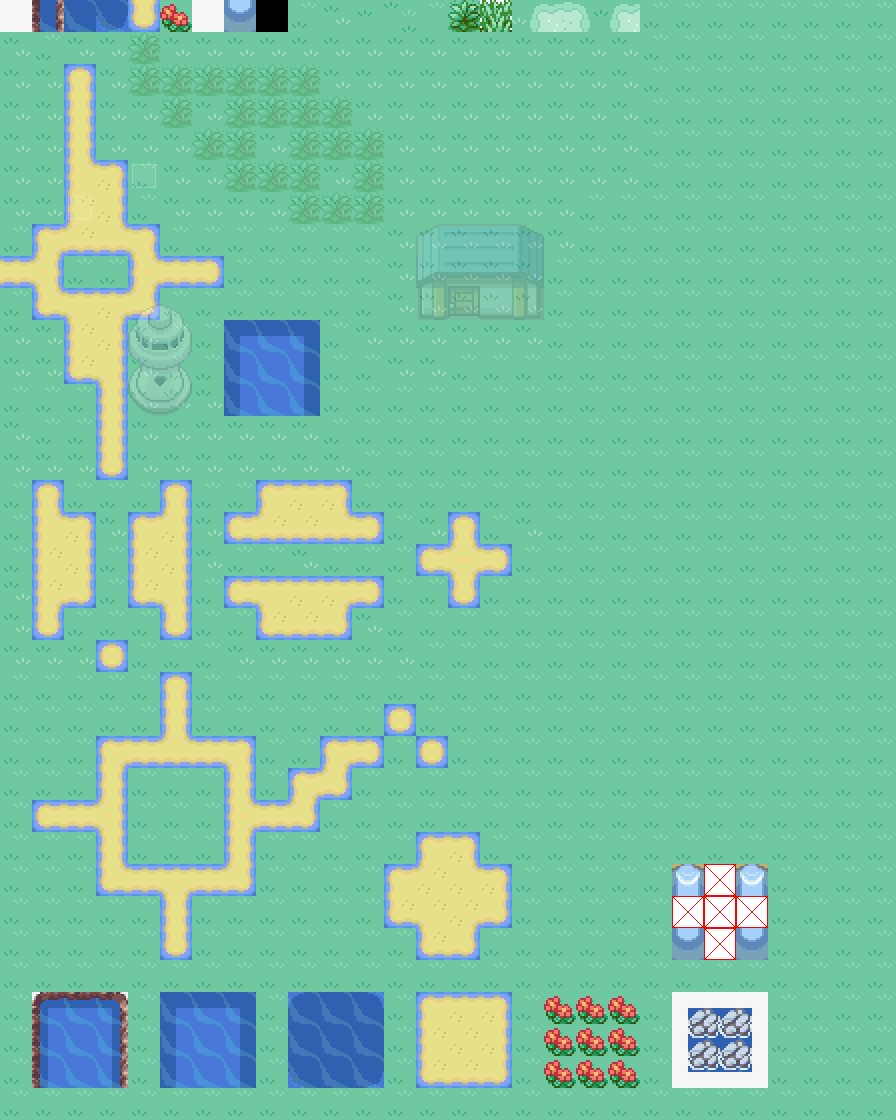
\includegraphics[width=.9\linewidth]{TestMap}










\end{document}
